%%%%%%%%%%%%%%%%%%%%%%%%%%%%%%%%%%%%%%%%%
% Beamer Presentation
% LaTeX Template
% Version 1.0 (10/11/12)
%
% This template has been downloaded from:
% http://www.LaTeXTemplates.com
%
% License:
% CC BY-NC-SA 3.0 (http://creativecommons.org/licenses/by-nc-sa/3.0/)
%
%%%%%%%%%%%%%%%%%%%%%%%%%%%%%%%%%%%%%%%%%

%----------------------------------------------------------------------------------------
%	PACKAGES AND THEMES
%----------------------------------------------------------------------------------------

\documentclass{beamer}

\mode<presentation> {

% The Beamer class comes with a number of default slide themes
% which change the colors and layouts of slides. Below this is a list
% of all the themes, uncomment each in turn to see what they look like.

%\usetheme{default}
%\usetheme{AnnArbor}
%\usetheme{Antibes}
%\usetheme{Bergen}
%\usetheme{Berkeley}
\usetheme{Berlin}
%\usetheme{Boadilla}
%\usetheme{CambridgeUS}
%\usetheme{Copenhagen}
%\usetheme{Darmstadt}
%\usetheme{Dresden}
%\usetheme{Frankfurt}
%\usetheme{Goettingen}
%\usetheme{Hannover}
%\usetheme{Ilmenau}
%\usetheme{JuanLesPins}
%\usetheme{Luebeck}
%\usetheme{Madrid}
%\usetheme{Malmoe}
%\usetheme{Marburg}
%\usetheme{Montpellier}
%\usetheme{PaloAlto}
%\usetheme{Pittsburgh}
%\usetheme{Rochester}
%\usetheme{Singapore}
%\usetheme{Szeged}
%\usetheme{Warsaw}

% As well as themes, the Beamer class has a number of color themes
% for any slide theme. Uncomment each of these in turn to see how it
% changes the colors of your current slide theme.

%\usecolortheme{albatross}
%\usecolortheme{beaver}
%\usecolortheme{beetle}
%\usecolortheme{crane}
%\usecolortheme{dolphin}
%\usecolortheme{dove}
%\usecolortheme{fly}
%\usecolortheme{lily}
%\usecolortheme{orchid}
%\usecolortheme{rose}
%\usecolortheme{seagull}
%\usecolortheme{seahorse}
%\usecolortheme{whale}
%\usecolortheme{wolverine}

%\setbeamertemplate{footline} % To remove the footer line in all slides uncomment this line
%\setbeamertemplate{footline}[page number] % To replace the footer line in all slides with a simple slide count uncomment this line

%\setbeamertemplate{navigation symbols}{} % To remove the navigation symbols from the bottom of all slides uncomment this line
\setbeamertemplate{caption}[numbered]
}

\usepackage[utf8]{inputenc}
\usepackage[portuguese]{babel}
\usepackage{graphicx} % Allows including images
\usepackage{booktabs} % Allows the use of \toprule, \midrule and \bottomrule in tables
\usepackage{caption}
\usepackage{subcaption}
\usepackage{float}
\usepackage{multirow} 
\usepackage{bigstrut}
\usepackage{textcomp}

\graphicspath{ {images/} } 

%----------------------------------------------------------------------------------------
%	TITLE PAGE
%----------------------------------------------------------------------------------------

\title[Desgaste de rodas ferroviárias]{Avaliação de desgaste de materiais de rodas ferroviárias forjadas com microestruturas perlítica e bainítica} % The short title appears at the bottom of every slide, the full title is only on the title page

\author{Henrique Abrantes Vitoi} % Your name
\institute[UFJF] % Your institution as it will appear on the bottom of every slide, may be shorthand to save space
{
Universidade Federal de Juiz de Fora \\ % Your institution for the title page
\medskip
\textit{vitoi.henrique@engenharia.ufjf.br} % Your email address
}
\date{\today} % Date, can be changed to a custom date

\begin{document}

\begin{frame}
\titlepage % Print the title page as the first slide
\end{frame}

\begin{frame}
\frametitle{Sumário} % Table of contents slide, comment this block out to remove it
{\tiny \tableofcontents} % Throughout your presentation, if you choose to use \section{} and \subsection{} commands, these will automatically be printed on this slide as an overview of your presentation
\end{frame}

%----------------------------------------------------------------------------------------
%	PRESENTATION SLIDES
%----------------------------------------------------------------------------------------

\section{Introdução} % Sections can be created in order to organize your presentation into discrete blocks, all sections and subsections are automatically printed in the table of contents as an overview of the talk

\subsection{Resumo}

\begin{frame}
	\frametitle{Análise de desgaste}
	
	\begin{itemize}
		\item Aço de composição próxima à eutetóide;
		\item Rodas forjadas;
		\item Microestruturas perlítica e bainítica
		\item Teste do tipo rolo contra disco.
	\end{itemize}
	
		
	\begin{minipage}[t]{0.4\textwidth}
		\begin{figure}
		\centering
		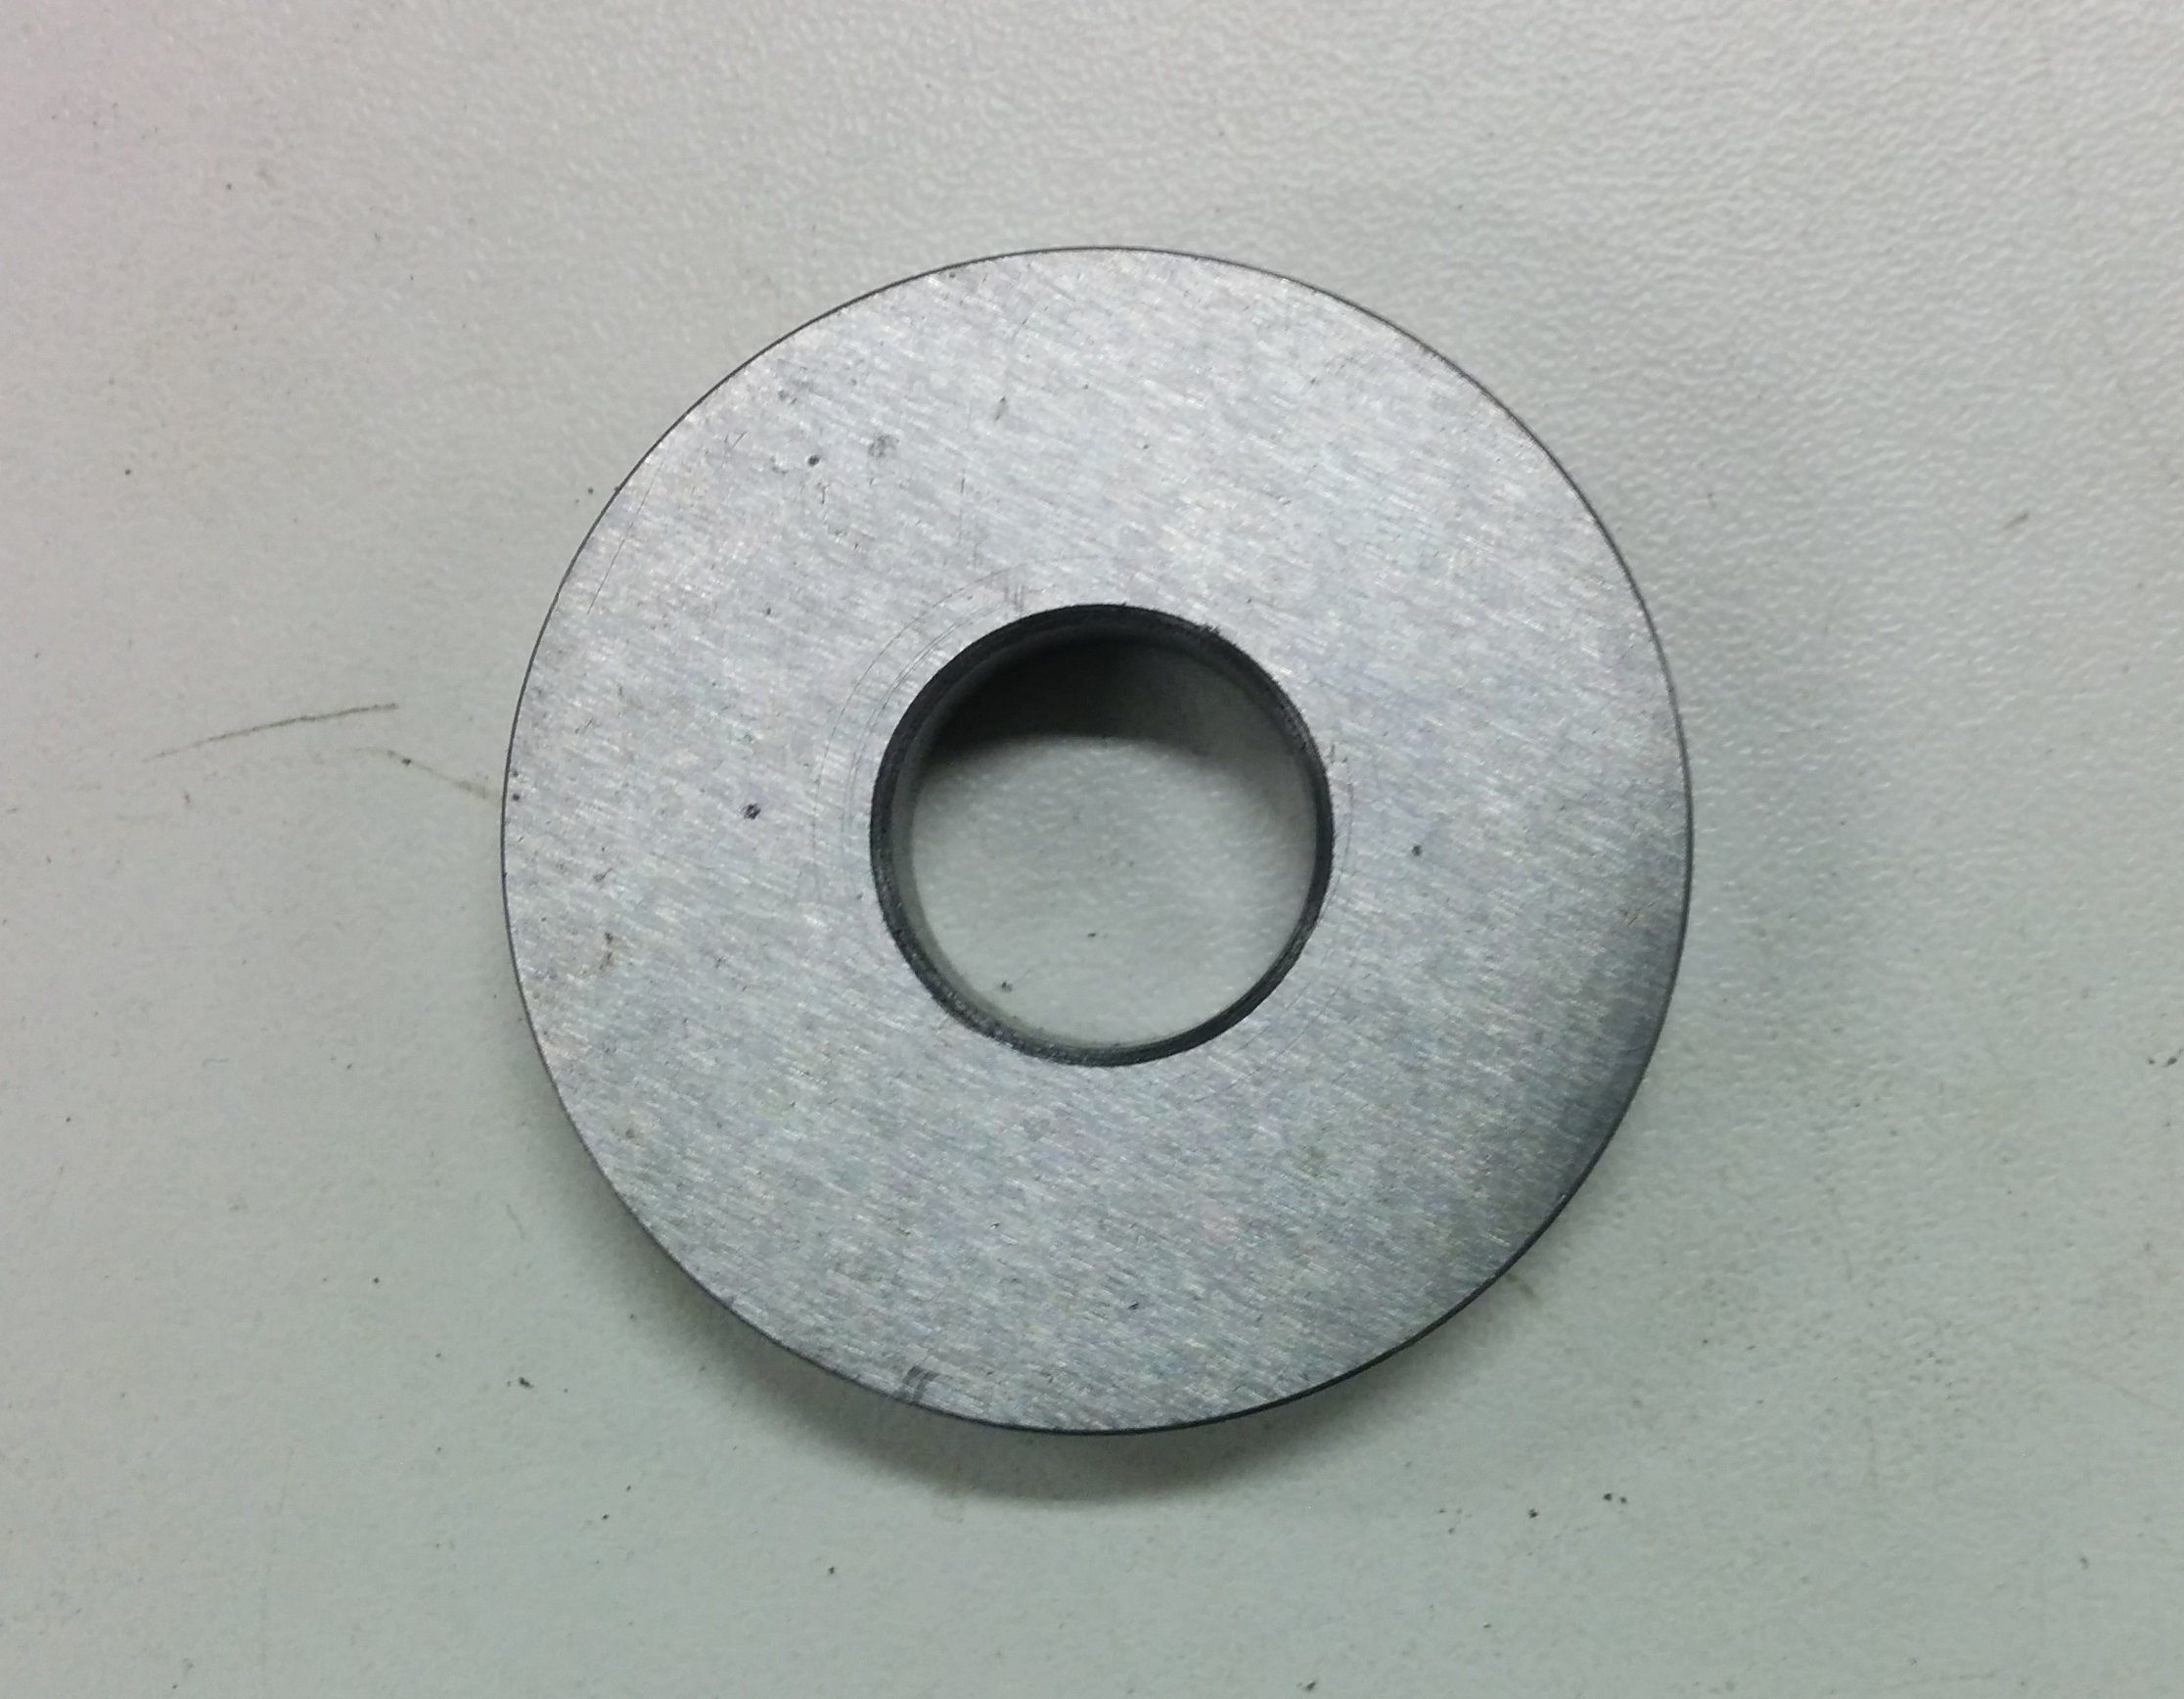
\includegraphics[width=0.8\textwidth]{amostra_perlita}
		\caption{Amostra perlítica.}
		\label{fig:amostra_perlita}
		\end{figure}
	\end{minipage}
	\hfill
	\begin{minipage}[t]{0.4\textwidth}
		\begin{figure}
		\centering
		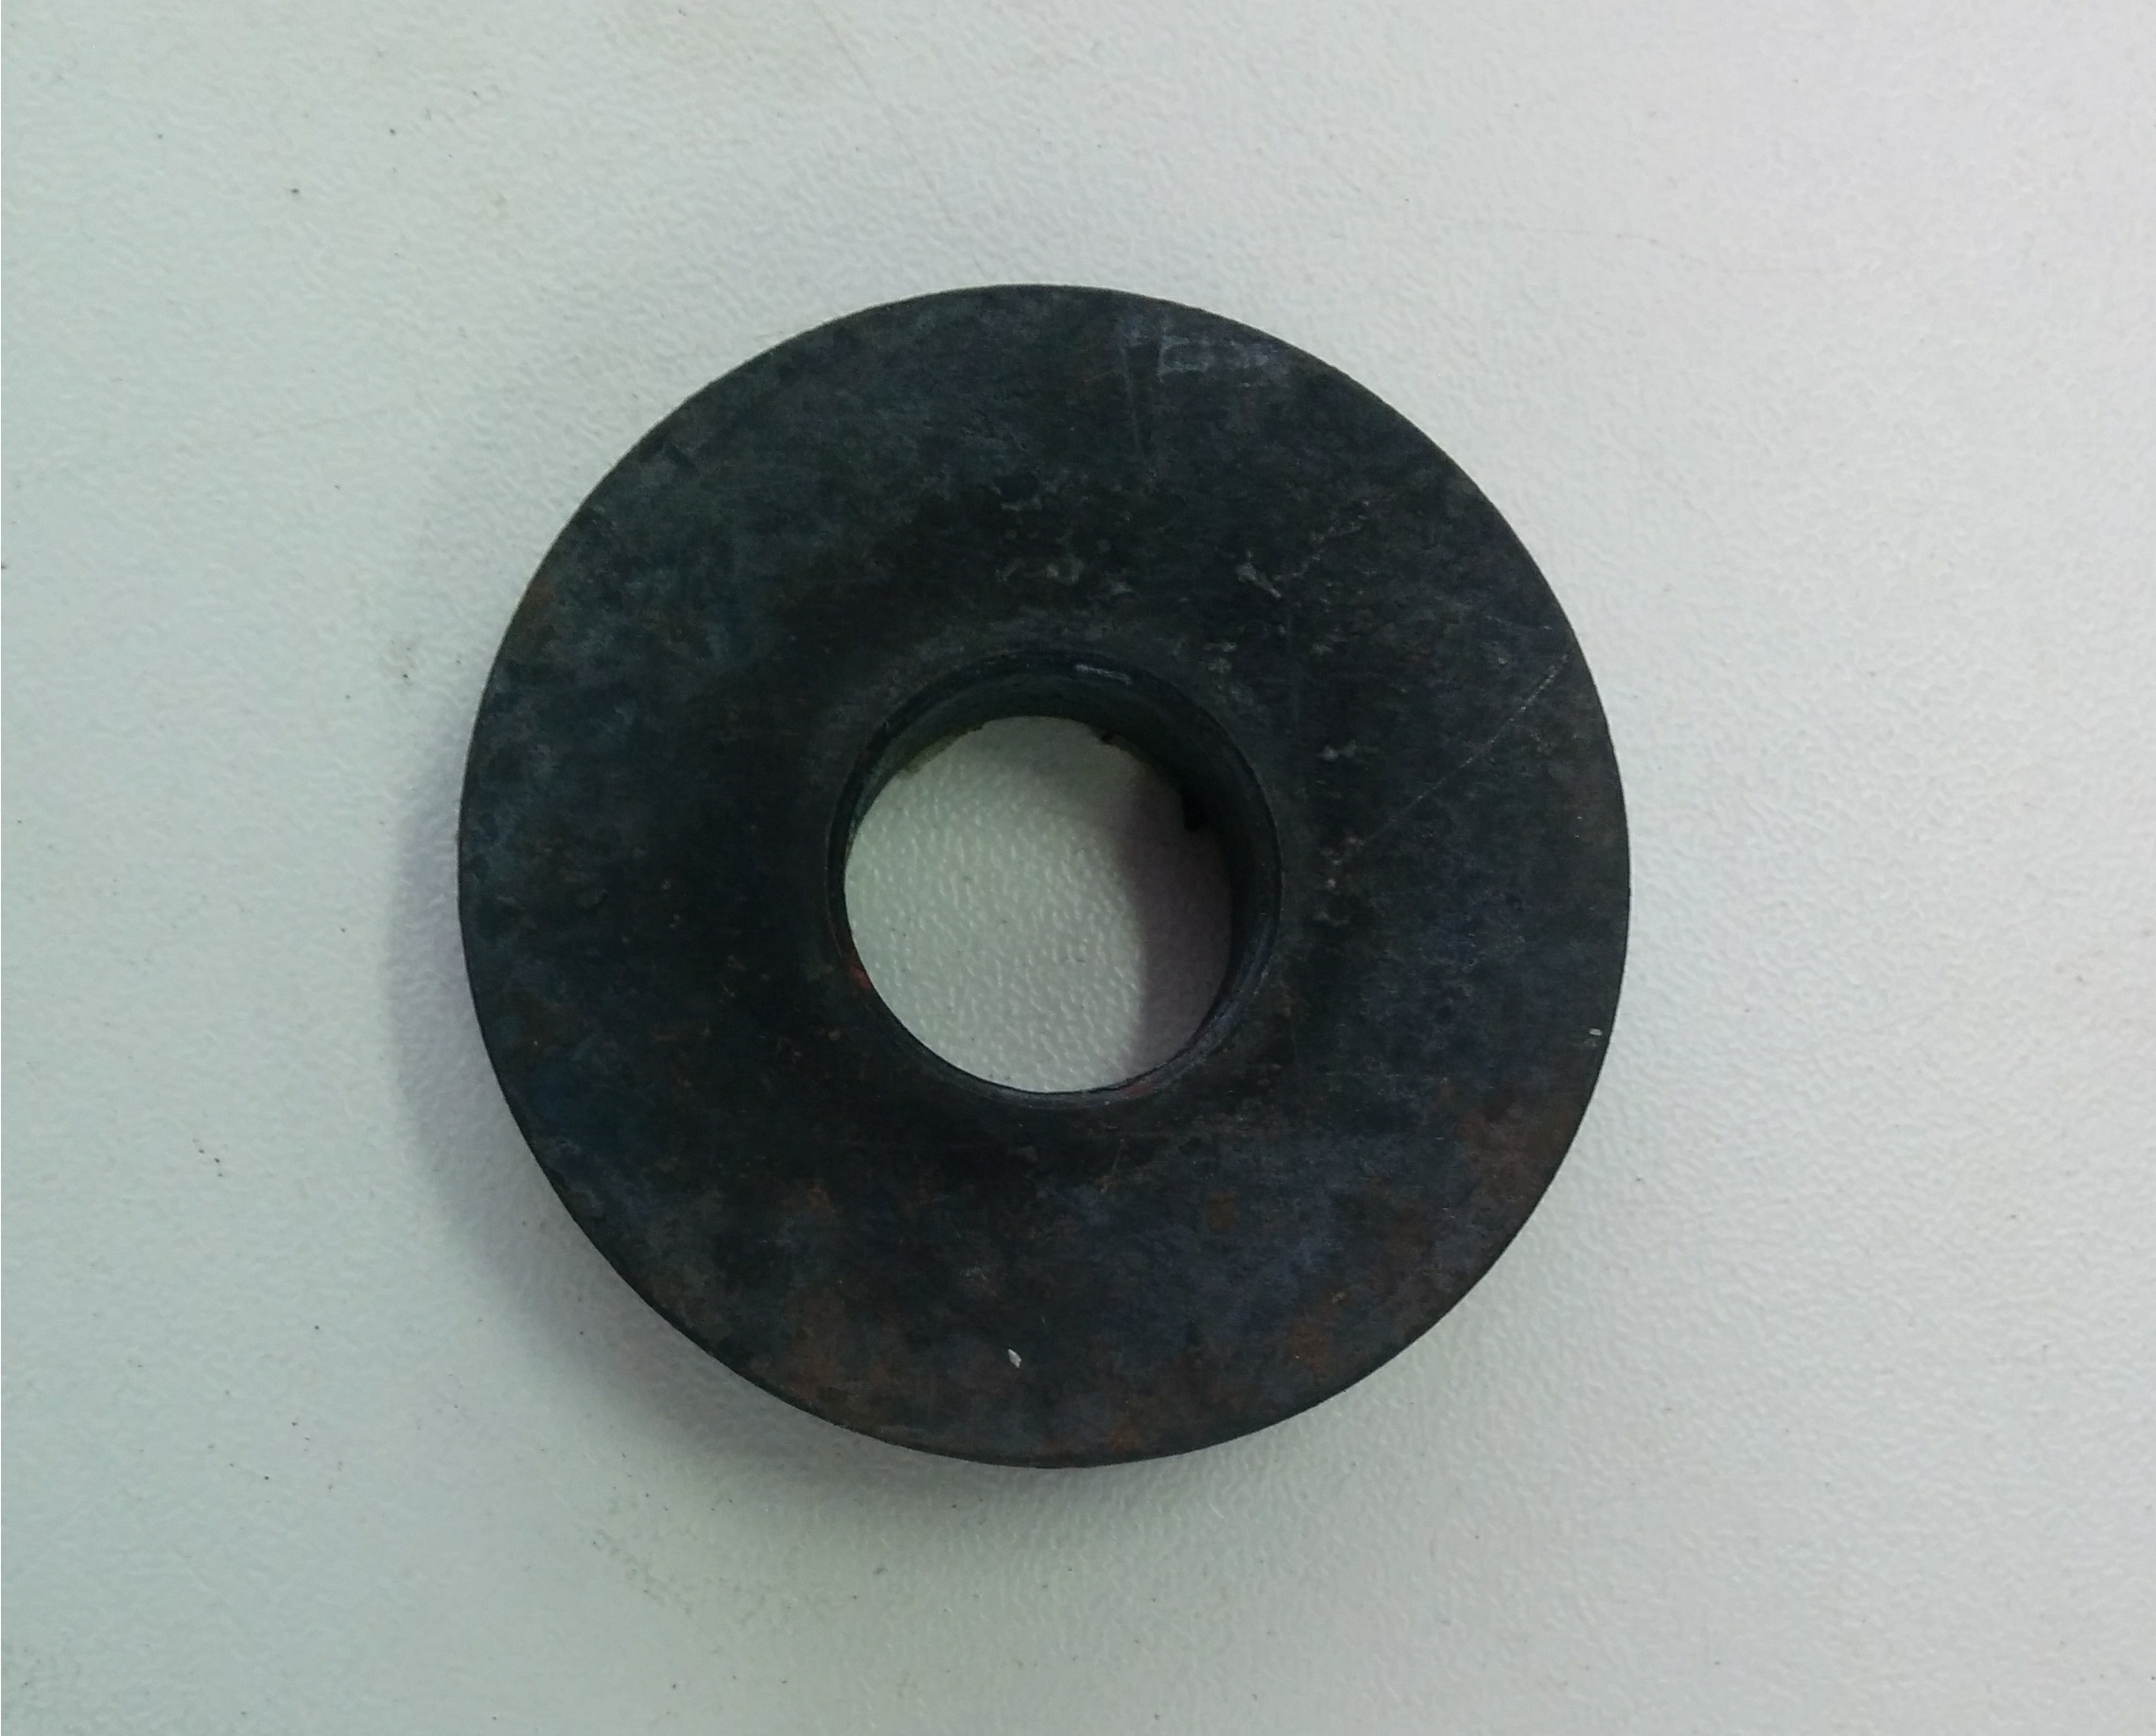
\includegraphics[width=0.8\textwidth]{amostra_bainita}
		\caption{Amostra bainítica.}
		\label{fig:amostra_bainita}
		\end{figure}
	\end{minipage}
	
\end{frame}

\begin{frame}
	\frametitle{Tribômetro}

	\begin{minipage}[t]{0.45\textwidth}	
		Funcionamento:
		\begin{itemize}
			\item Tribômetro do tipo rolo contra disco;
			\item Análise de desgaste por perda de massa.
		\end{itemize}
		
		Principais partes:
		\begin{enumerate}
		\item Rolo (corpo);
		\item Disco (contracorpo);
		\item Pino de apoio de carga.
		\end{enumerate}
	\end{minipage}
	\hfill
	\begin{minipage}[t]{0.45\textwidth}
		\begin{figure}
			\centering
			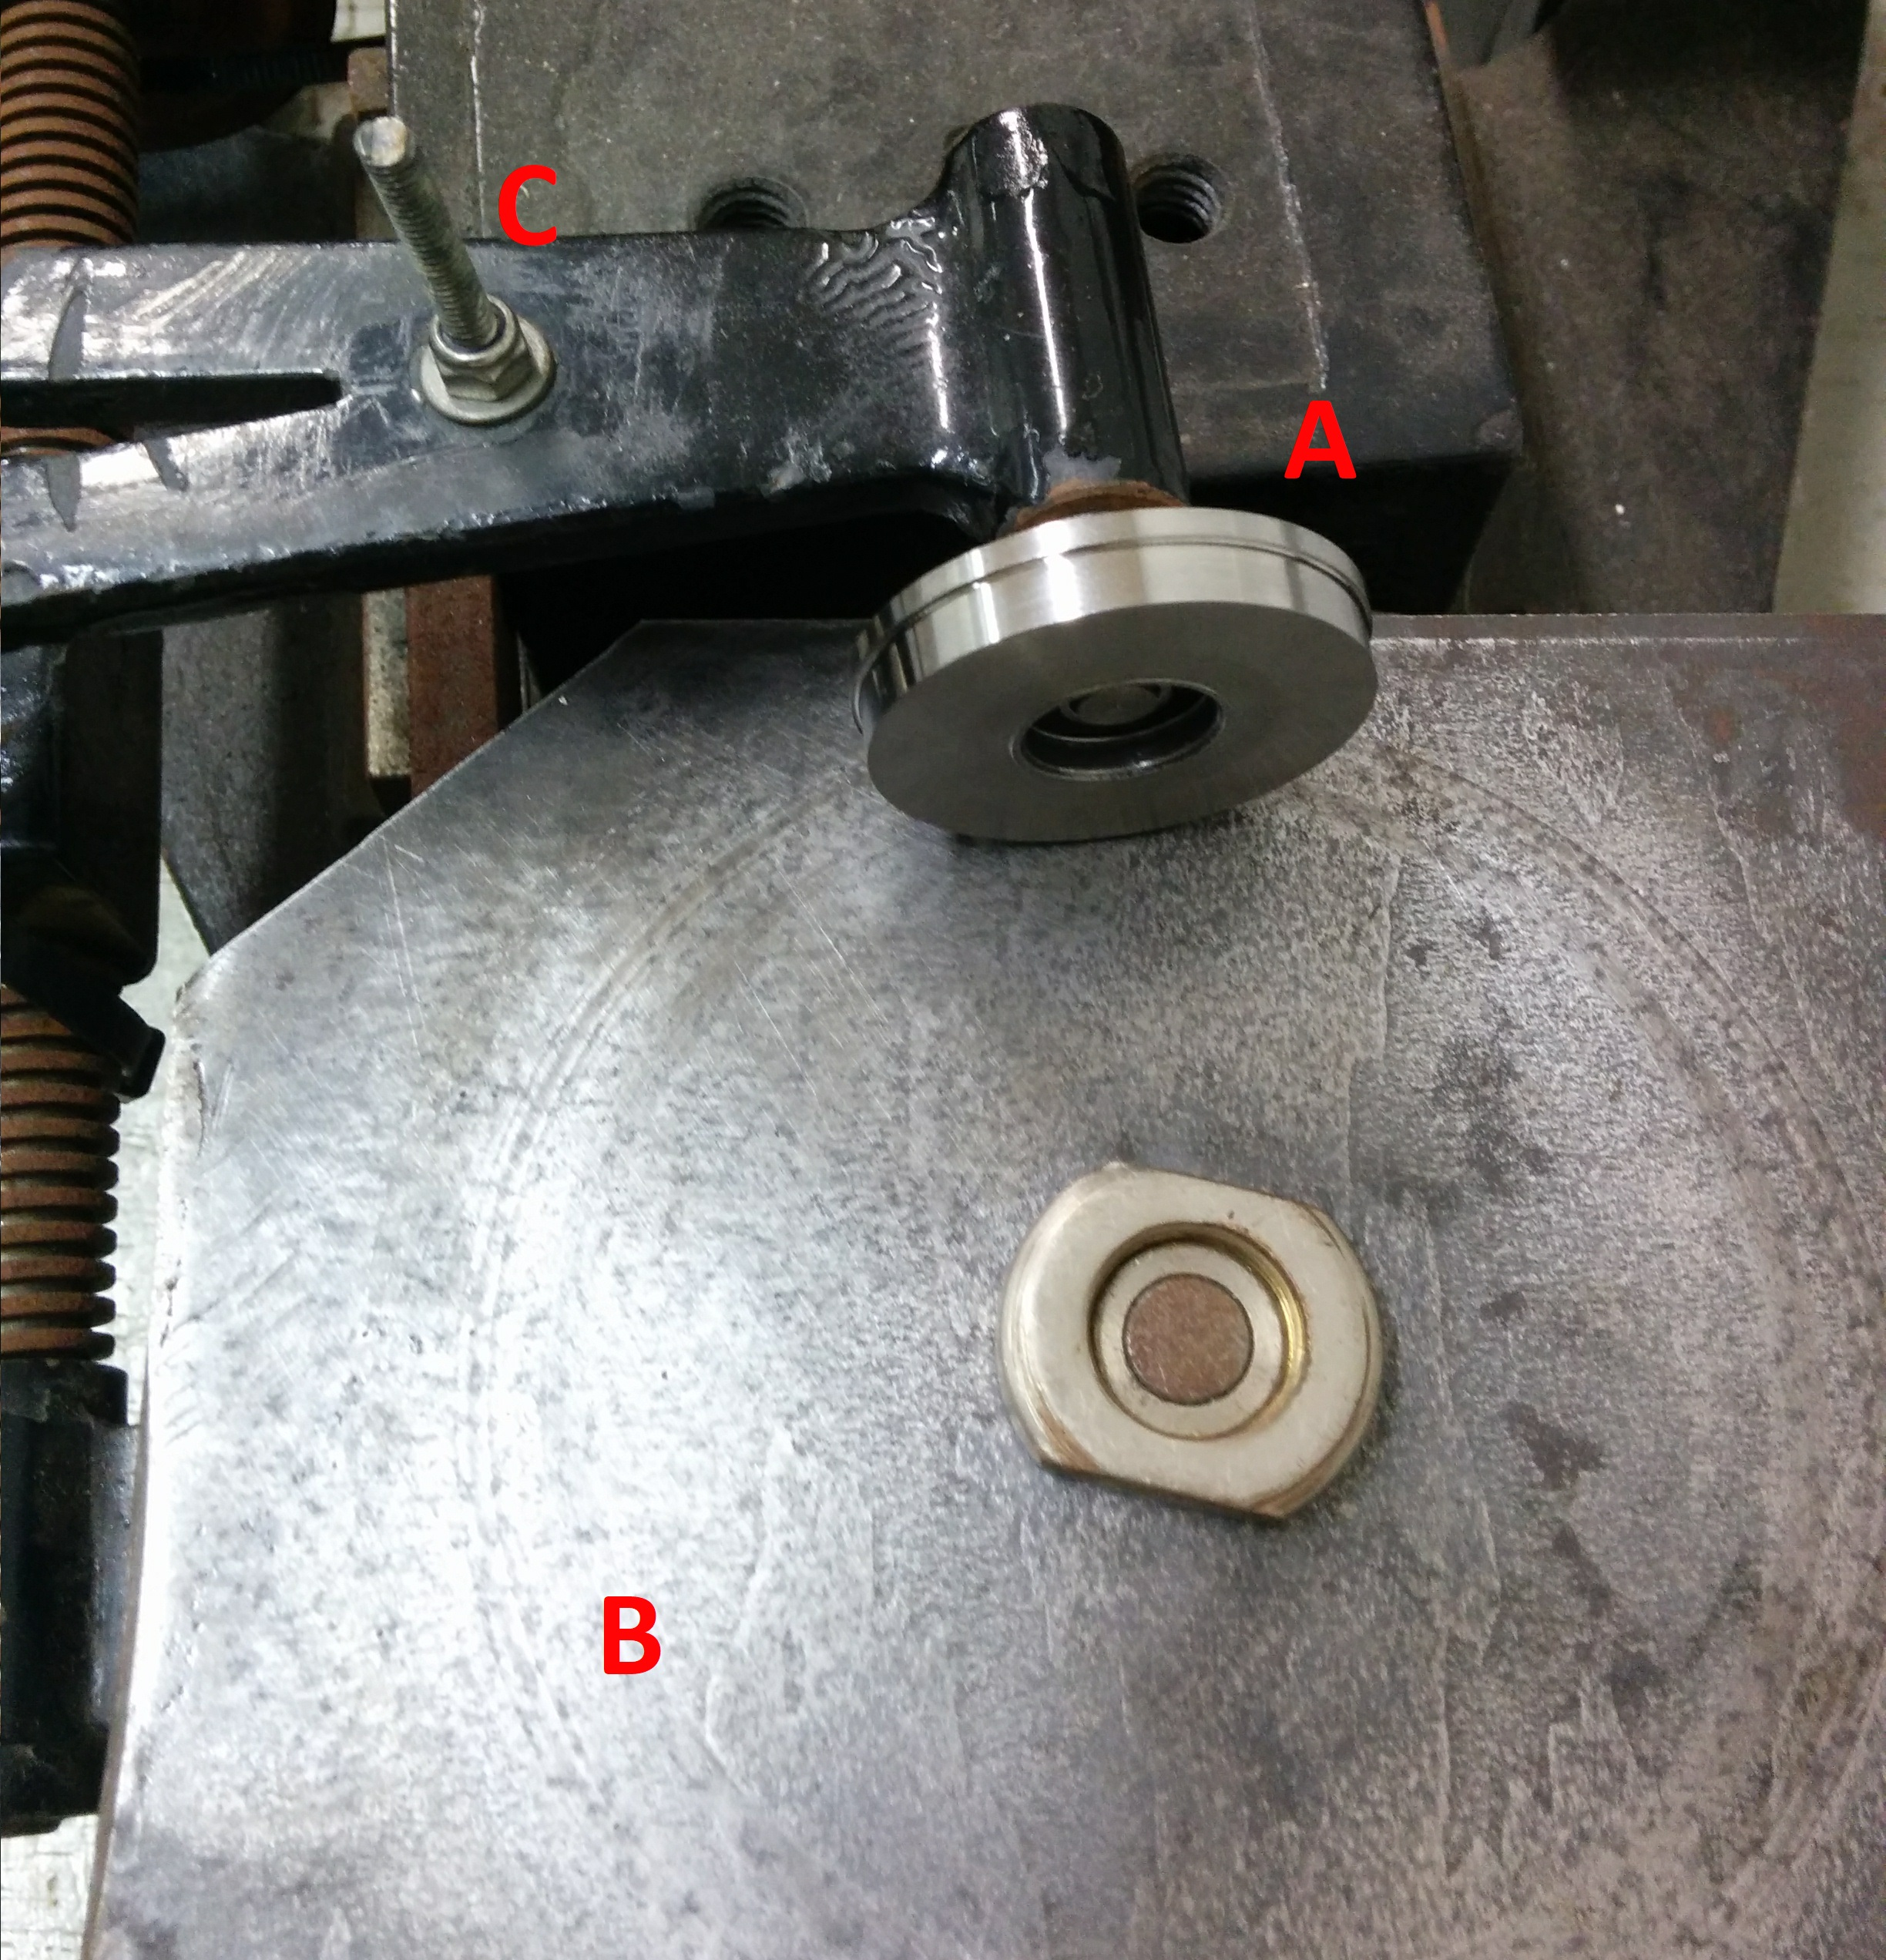
\includegraphics[width=1\textwidth]{tribometro_partes}
			\caption{Partes do tribômetro.}
			\label{fig:tribometro_partes}
		\end{figure}
	\end{minipage}

\end{frame}

\begin{frame}
\frametitle{Tribômetro em funcionamento}
\begin{figure}
	\centering
	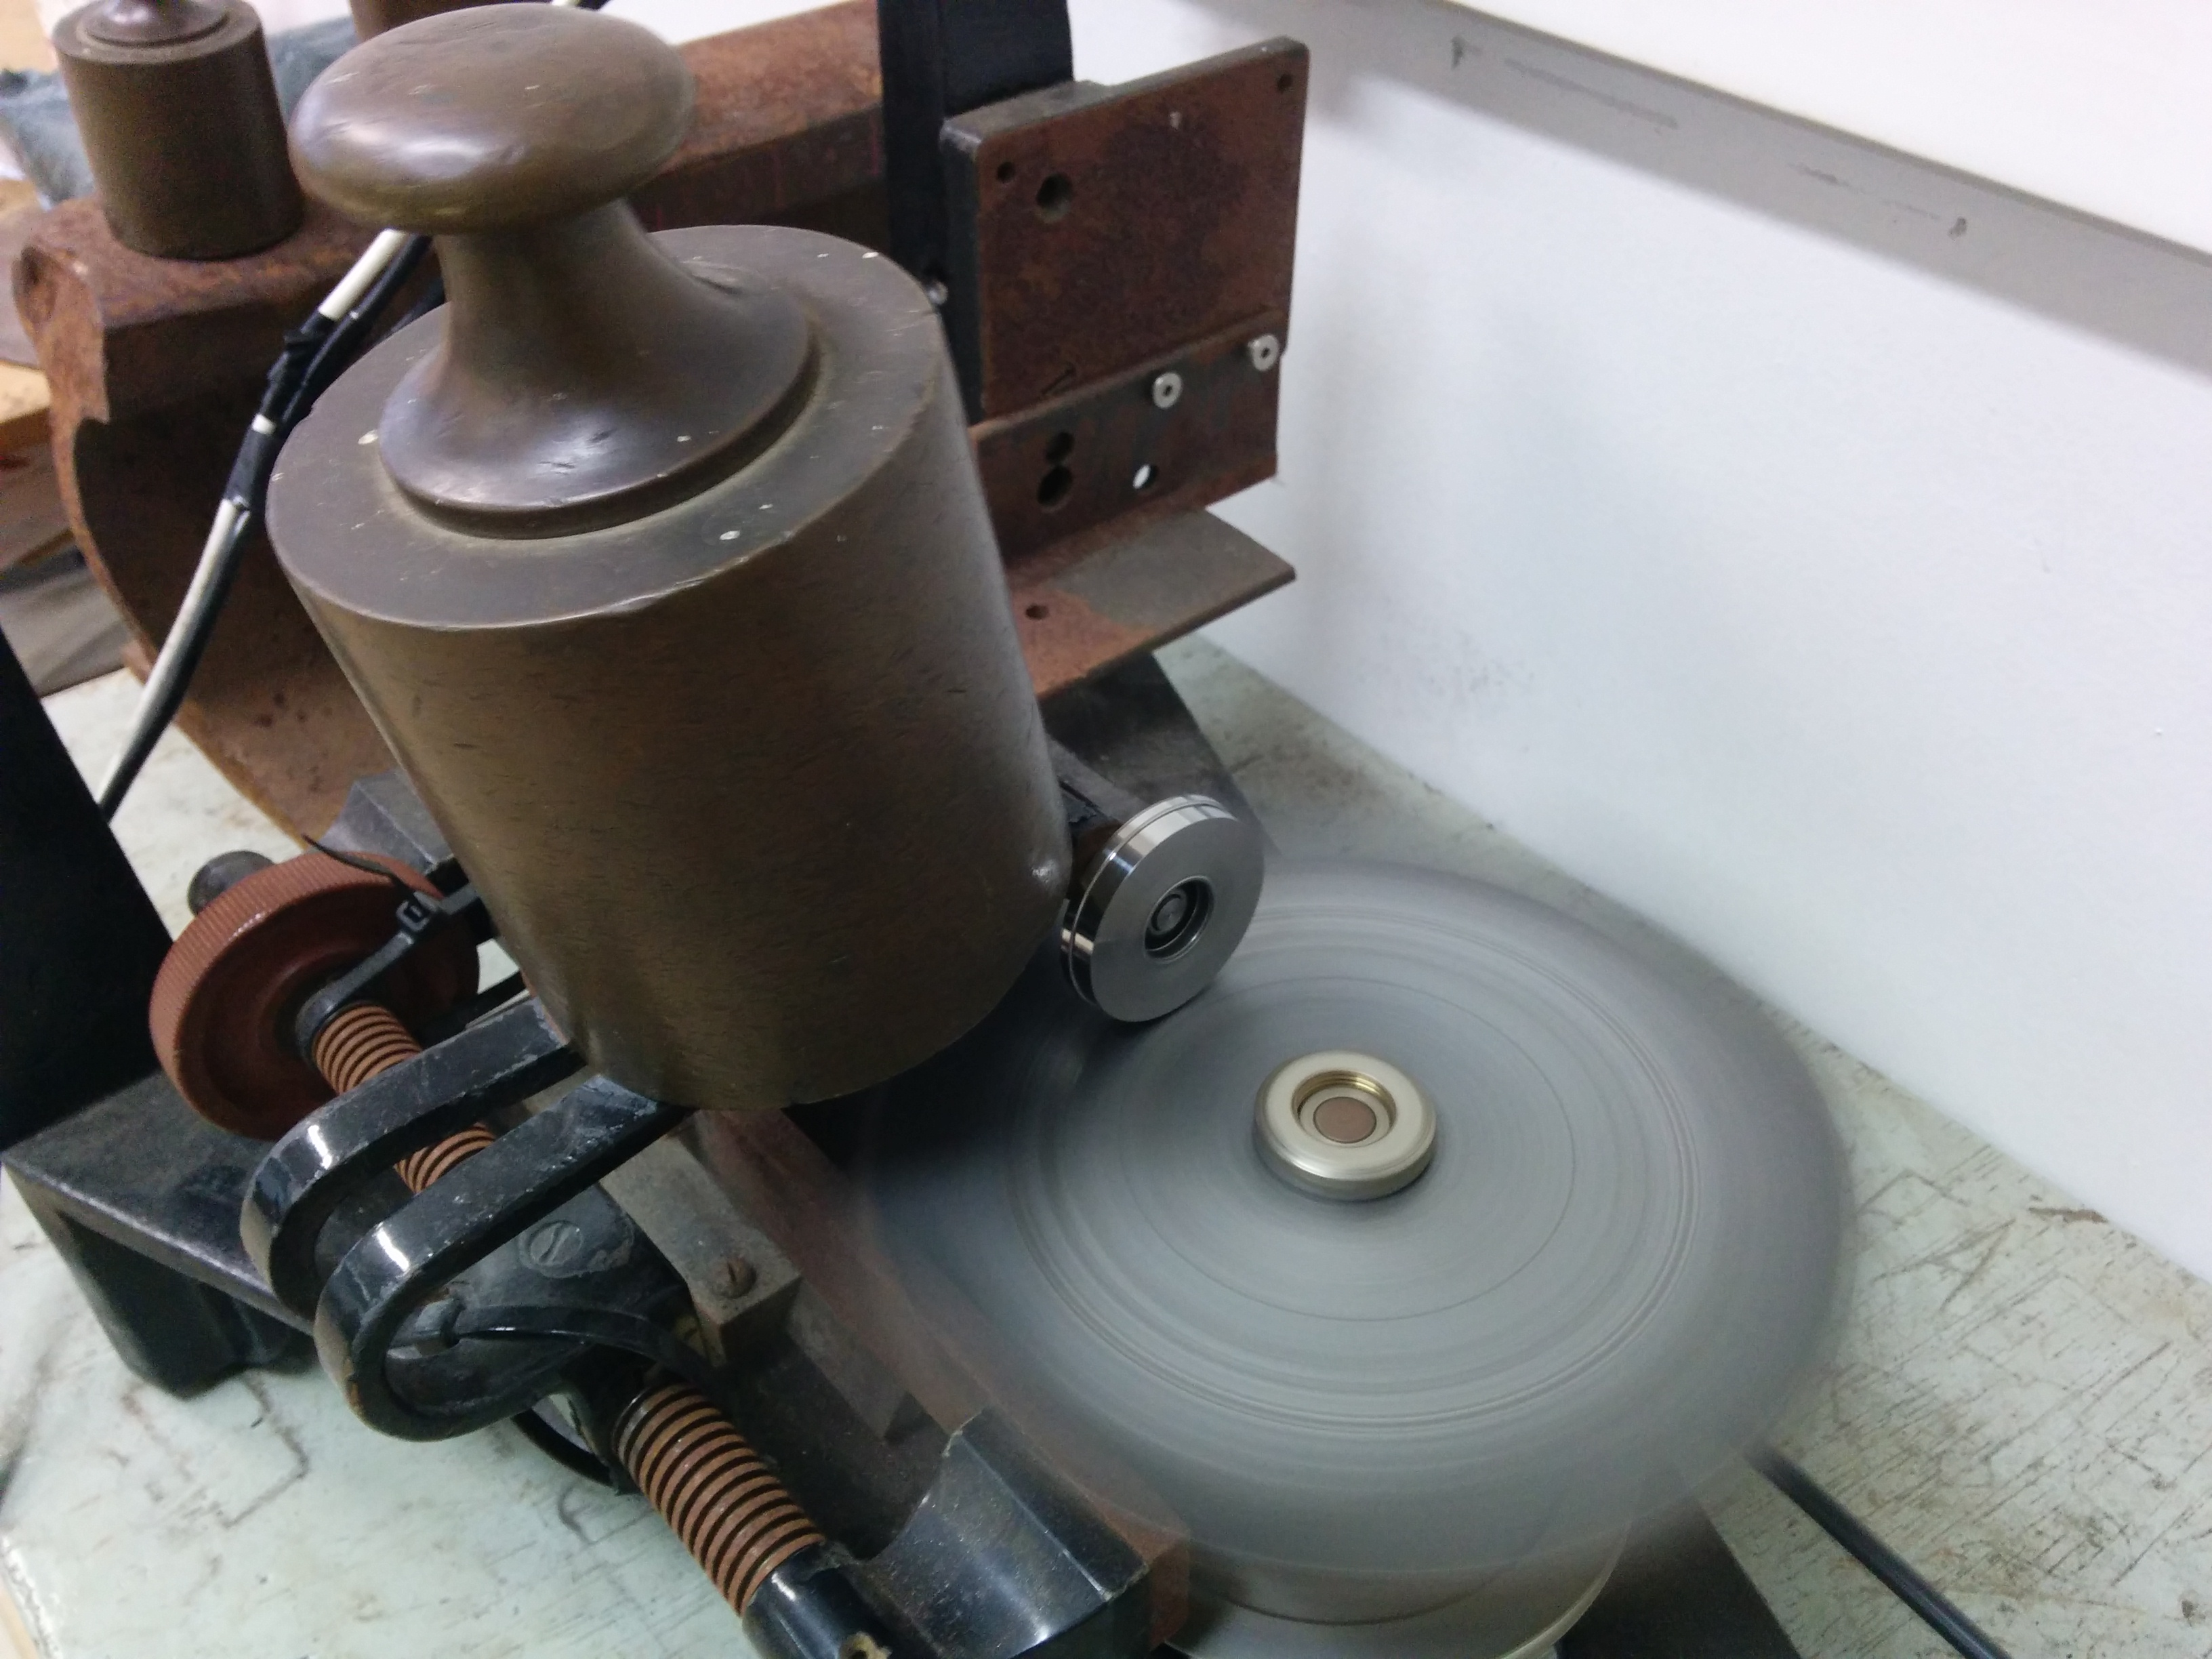
\includegraphics[width=0.65\textwidth]{tribometro}
	\caption{Teste de desgaste em um tribômetro.}
	\label{fig:tribometro}
\end{figure}
\end{frame}


\subsection{Propósito do trabalho}

\begin{frame}
\frametitle{Redução de custos no setor ferroviário}
	\centering
	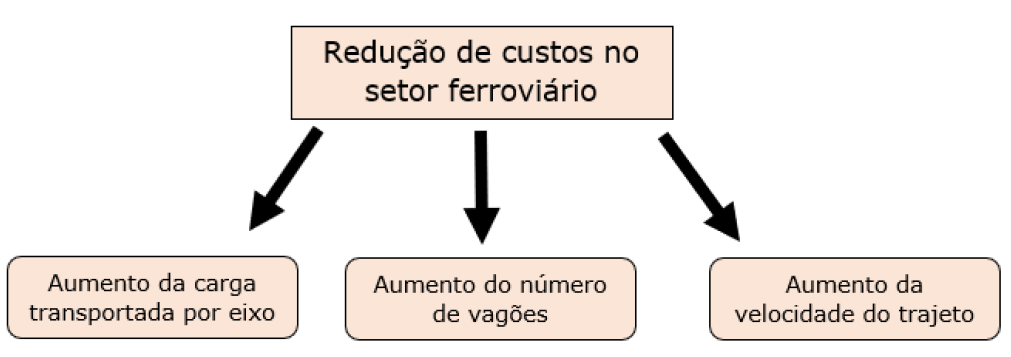
\includegraphics[width=1\textwidth]{custos}
\end{frame}

\begin{frame}
\frametitle{Redução de custos no setor ferroviário}
\centering
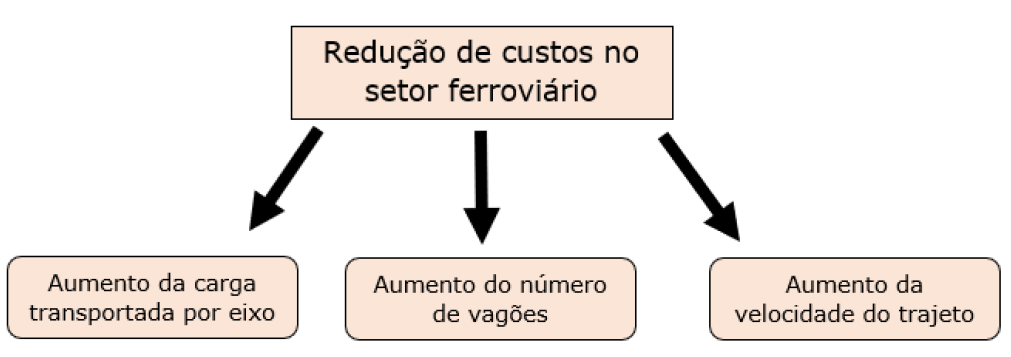
\includegraphics[width=1\textwidth]{custos}
\hfill
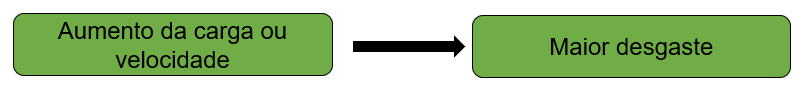
\includegraphics[width=1\textwidth]{custos2}
\end{frame}

\begin{frame}
\frametitle{Gasto com manutenções e outros}
O maior desgaste das partes mecânicas geram custos diretos e indiretos como:
\begin{enumerate}
	\item Manutenção corretiva;
\end{enumerate}
\end{frame}

\begin{frame}
\frametitle{Gasto com manutenções e outros}
O maior desgaste das partes mecânicas geram custo diretos e indiretos como:
\begin{enumerate}
	\item Manutenção corretiva;
	\item Manutenção preventiva;
\end{enumerate}
\end{frame}

\begin{frame}
\frametitle{Gasto com manutenções e outros}
O maior desgaste das partes mecânicas geram custo diretos e indiretos como:
\begin{enumerate}
	\item Manutenção corretiva;
	\item Manutenção preventiva;
	\item Acidentes;
\end{enumerate}
\end{frame}

\begin{frame}
\frametitle{Gasto com manutenções e outros}
O maior desgaste das partes mecânicas geram custo diretos e indiretos como:
\begin{enumerate}
	\item Manutenção corretiva;
	\item Manutenção preventiva;
	\item Acidentes;
	\item Imagem da empresa;
\end{enumerate}
\end{frame}

\begin{frame}
\frametitle{Gasto com manutenções e outros}
O maior desgaste das partes mecânicas geram custo diretos e indiretos como:
\begin{enumerate}
	\item Manutenção corretiva;
	\item Manutenção preventiva;
	\item Acidentes;
	\item Imagem da empresa;
	\item ...
\end{enumerate}
\end{frame}

\begin{frame}
\frametitle{Importância da redução de custos}

\begin{itemize}
	\item Para empresas operando no nicho de logística em ferrovias, a redução de custos é essencial.
	\item Garante a competitividade de seus produtos e serviços.
	\item Determina a sobrevivência da empresa no mercado, cada vez mais competitivo.
	
\end{itemize}


\end{frame}


%------------------------------------------------
\subsection{Objetivos}

\begin{frame}

\begin{block}{Análise das microestruturas}
	Analisar o comportamento em desgaste a seco de materiais de rodas forjadas de mesma composição química e dureza, porém com diferentes microestruturas: perlítica e bainítica.
\end{block}



\end{frame}
%------------------------------------------------
\begin{frame}

\begin{block}{Análise das microestruturas}
	Analisar o comportamento em desgaste a seco de materiais de rodas forjadas de mesma composição química e dureza, porém com diferentes microestruturas: perlítica e bainítica.
\end{block}

\begin{block}{Desgaste do aço eutetóide}
	Estudo de amostras de roda de aço de composição próxima a eutetóide, muito utilizadas nas aplicações de heavy haul, onde há altas cargas, tensões e esforços mecânicos envolvidos.
\end{block}

	

\end{frame}
%------------------------------------------------
\begin{frame}

\begin{block}{Análise das microestruturas}
	Analisar o comportamento em desgaste a seco de materiais de rodas forjadas de mesma composição química e dureza, porém com diferentes microestruturas: perlítica e bainítica.
\end{block}

\begin{block}{Desgaste do aço eutetóide}
	Estudo de amostras de roda de aço de composição próxima a eutetóide, muito utilizadas nas aplicações de heavy haul, onde há altas cargas, tensões e esforços mecânicos envolvidos.

\end{block}

\begin{block}{Orientar empresas}
	Orientar e sugerir aos fabricantes na indústria ferroviária e empresas operantes em ferrovias sobre qual microestrutura apresenta melhor comportamento em desgaste.
	
\end{block}
\end{frame}

%------------------------------------------------





\section{Fundamentação teórica}

\subsection{Tribologia}
\begin{frame}
\frametitle{Conceito}
	\begin{itemize}
		
	\item A tribologia é a ciência que estuda os fenômenos de fricção, desgaste e lubrificação
	
	\item A análise da interação entre a roda e o trilho ferroviário também é escopo de estudo da tribologia.
	
\end{itemize}
\end{frame}

\begin{frame}
\frametitle{Fricção e movimentos relativos}
A força de fricção pode ser definida como a resistência encontrada por um corpo ao se mover sobre outro. A fricção engloba duas importantes classes de movimento relativo: 
\begin{enumerate}
	\item Movimento de rolamento;
	\item Movimento de deslizamento.
	
	\begin{figure}
		\centering
		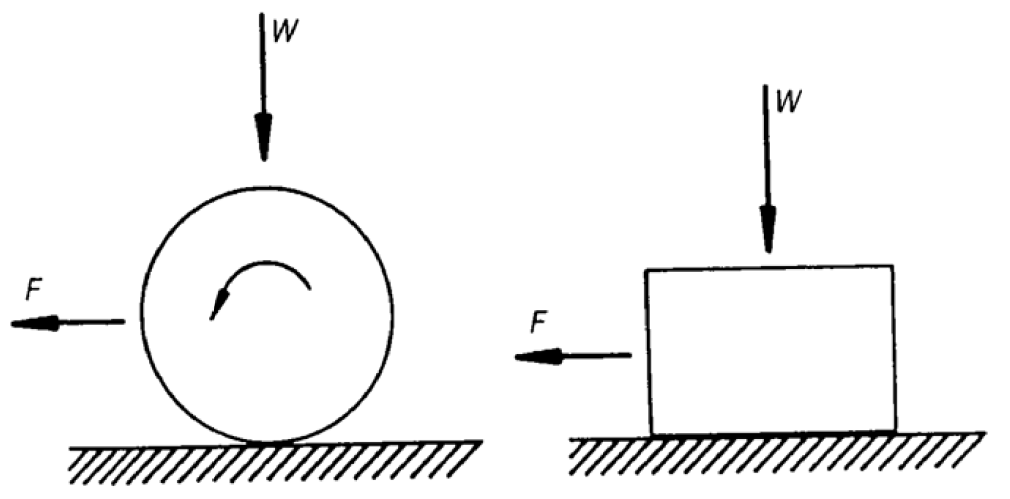
\includegraphics[width=0.5\textwidth]{rolamento_deslizamento}
		\caption{Movimentos de rolamento e deslizamento.}
		\label{fig:rolamento_deslizamento}
	\end{figure}
\end{enumerate}
\end{frame}

\begin{frame}
\frametitle{Análise de desgaste por deslizamento e rolamento}

\begin{columns}[c] % The "c" option specifies centered vertical alignment while the "t" option is used for top vertical alignment
\column{.5\textwidth} % Left column and width
	\begin{itemize}
		\item Experimentações são feitas para estudar o desgaste por deslizamento e rolamento.
		\item Investigações em laboratório simulam aplicações práticas com diferentes variáveis.
		\item Visa a obtenção de taxas de desgaste e coeficientes de fricção para cada caso.
	\end{itemize}

\column{.5\textwidth} % Right column and width]
\begin{figure}
	\centering
	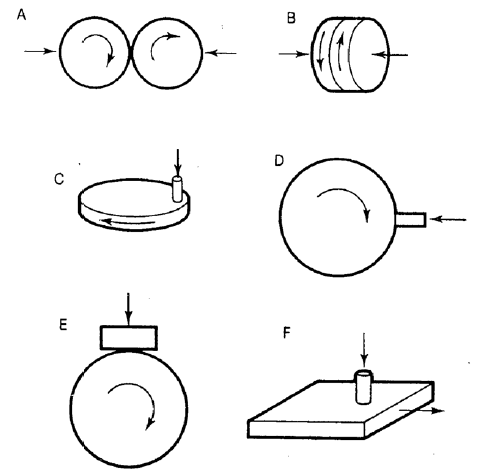
\includegraphics[width=0.8\textwidth]{testes_desgaste}
	\caption{Geometrias empregadas em testes de desgaste.}
	\label{fig:testes_desgaste}
\end{figure}
\end{columns}


\end{frame}

\begin{frame}
\frametitle{A equação de desgaste de Archard}
A taxa de desgaste é baseada a partir de uma simples teoria do desgaste: a equação de desgaste de Archard.


\begin{equation} \label{eq:archard}
Q = K\frac{W}{H}
\end{equation}

Onde:\\
{\scriptsize Q: Taxa de desgaste (Volume de  material perdido com o atrito);\\
K: Constante de severidade do desgaste;\\
W: Carga aplicada para o contato entre os corpos;\\
H: Dureza do material mais macio.\\}


\end{frame}




\subsection{Rodas ferroviárias}

\begin{frame}

\frametitle{Características relevantes da roda}



\begin{figure}
	\centering
	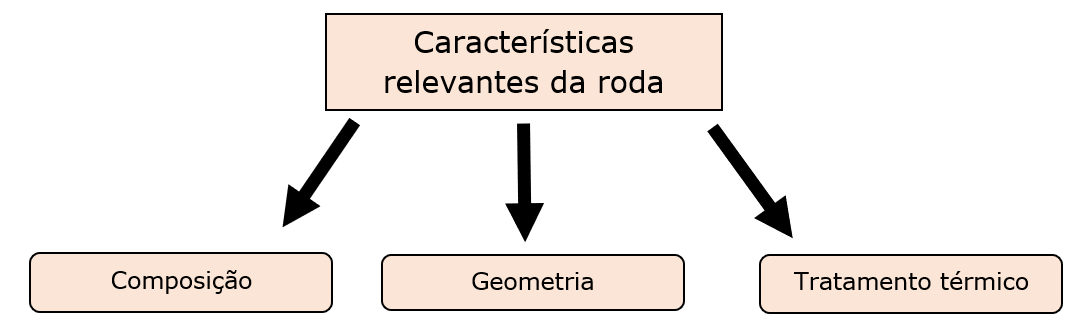
\includegraphics[width=0.8\textwidth]{caracteristicas_roda}
	\caption{Características relevantes da roda ao se analisar desgaste.}
	\label{fig:caracteristicas_roda}
\end{figure}


Cada vez mais pesquisas são realizadas a fim de se aprimorar o sistema roda-trilho. 


\end{frame}

\begin{frame}

\frametitle{Análise do impacto do tratamento térmico no desempenho da roda}



\begin{figure}
	\centering
	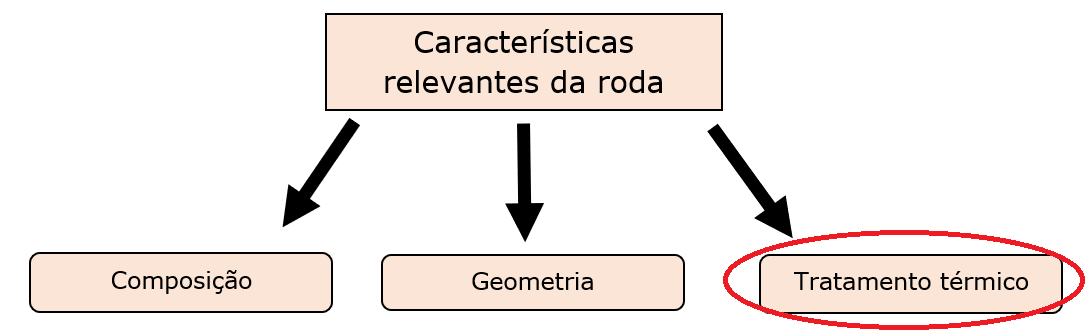
\includegraphics[width=1\textwidth]{caracteristicas_roda_circ}
	\caption{Características relevantes da roda ao se analisar desgaste.}
	\label{fig:caracteristicas_roda_circ}
\end{figure}



\end{frame}


\subsection{Ligas Ferro-Carbono}

\begin{frame}
\frametitle{Microestruturas do aço}
\begin{itemize}
	\item Dependendo da temperatura, da composição e do tratamento térmico utilizado, o aço pode apresentar diferentes microestruturas.
\end{itemize}

\begin{figure}
	\centering
	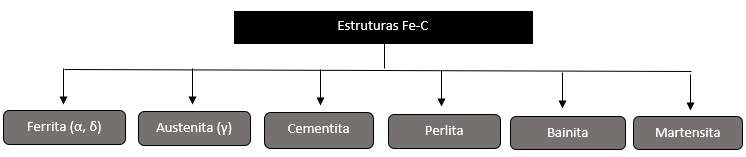
\includegraphics[width=1\textwidth]{alotropia}
	\caption{Algumas microestruturas comuns em aços.}
	\label{fig:alotropia}
\end{figure}

\end{frame}

\begin{frame}
\frametitle{ Propriedades das microestruturas}
\begin{itemize}
	\item As propriedades de cada microestrutura são bem distintas entre si, apresentando cada uma aplicações diferentes.
\end{itemize}	
	\begin{table}[H]
		\centering
		\caption{Propriedades mecânicas dos microconstituintes do aço.}
		\resizebox{\textwidth}{!}{%
			\begin{tabular}{|c|c|c|c|c|}
				\hline
				\multirow{2}{*}{\textbf{Constituinte}} & \multicolumn{2}{c|}{\textbf{Limite de resistência à tração}} & \multicolumn{1}{c|}{\multirow{2}{*}{\textbf{Alongamento em 2''\newline{}(\%)}}} & \multirow{2}{*}{\textbf{Dureza Brinell}} \bigstrut\\
				\cline{2-3}               & \textbf{$kgf/mm^2$} & \textbf{MPa} &            &  \bigstrut\\
				\hline
				Ferrita    & 35         & 340        & cerca de 40 & 90 \bigstrut[t]\\
				Perlita    & 85         & 830        & cerca de 10 & 250-300 \\
				Cementita  & 3          & 30         & 0          & 650 \bigstrut[b]\\
				\hline
			\end{tabular}%
		}
		\label{tab:propriedades_aco}%
		
	\end{table}%




\end{frame}

\begin{frame}
\frametitle{Perlita e Bainita}


	\centering
	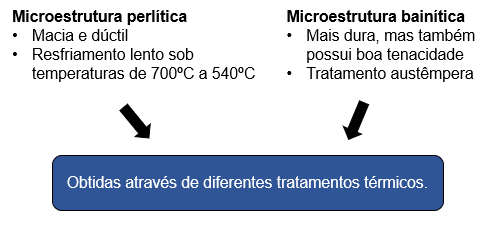
\includegraphics[width=1\textwidth]{perl_bain}



\end{frame}





%------------------------------------------------
\section{Metodologia}
%------------------------------------------------
\subsection{Preparação das amostras}
\begin{frame}
\frametitle{Local de retirada do material}
\begin{columns}[c] % The "c" option specifies centered vertical alignment while the "t" option is used for top vertical alignment
	\column{.6\textwidth} % Left column and width
	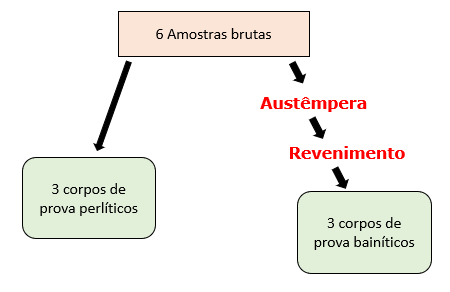
\includegraphics[width=1\textwidth]{amostrass}
	
	\column{.4\textwidth} % Right column and width]
	\begin{figure}
		\centering
		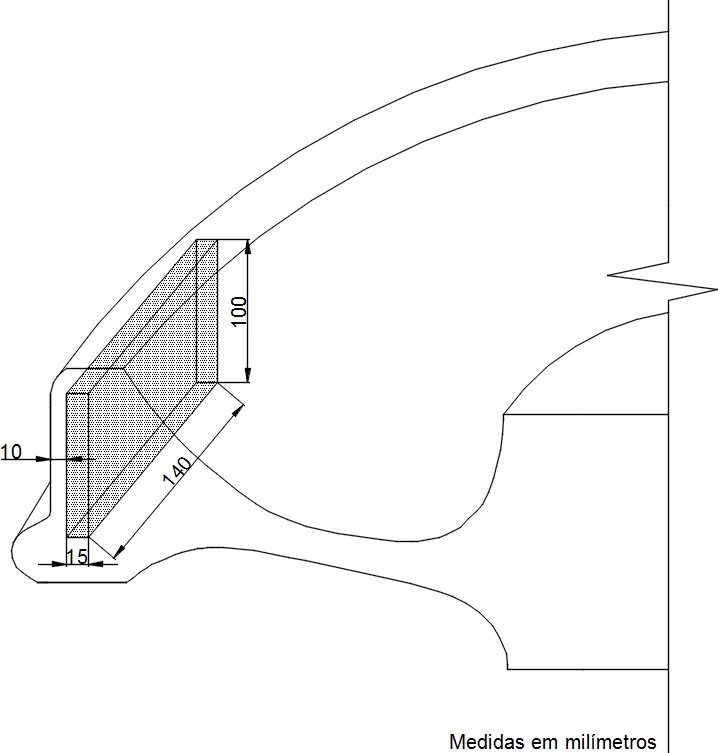
\includegraphics[width=0.8\textwidth]{secao_roda}
		\caption{Desenho esquematizado do local de retirada do material.}
		\label{fig:secao_roda}
	\end{figure}
\end{columns}
\end{frame}

\begin{frame}
\frametitle{Espectrometria do material}
	\begin{table}[H]
	\centering
	\caption{Composição química das amostras via Espectrômetro de Emissão Óptica}
	\resizebox{0.3\textwidth}{!}{%
		\begin{tabular}{|p{8em}|c|}
			\hline
			\textbf{Elementos} & \multicolumn{1}{p{8em}|}{\textbf{Identificação das Amostras}} \bigstrut\\
			\hline
			Carbono (\%) & 0,760 \bigstrut\\
			\hline
			Manganês (\%) & 0,846 \bigstrut\\
			\hline
			Silício (\%) & 0,906 \bigstrut\\
			\hline
			Fósforo(\%) & 0,014 \bigstrut\\
			\hline
			Enxofre(\%) & 0,017 \bigstrut\\
			\hline
			Cromo (\%) & 0,096 \bigstrut\\
			\hline
			Molibdênio (\%) & 0,032 \bigstrut\\
			\hline
			Níquel (\%) & 0,022 \bigstrut\\
			\hline
			Alumínio (\%) & 0,004 \bigstrut\\
			\hline
			Cobre (\%) & 0,034 \bigstrut\\
			\hline
			Boro (\%)  & 0,000 \bigstrut\\
			\hline
			Vanádio (\%) & 0,002 \bigstrut\\
			\hline
			Cobalto (\%) & 0,007 \bigstrut\\
			\hline
		\end{tabular}%
	}
	\label{tab:composicao}%
\end{table}%
\end{frame}

\begin{frame}
\frametitle{Preparação das rodas perlíticas}
\begin{columns}[c] % The "c" option specifies centered vertical alignment while the "t" option is used for top vertical alignment
	\column{.6\textwidth} % Left column and width
	\begin{itemize}
		\item Usinagem do material para a fabricação de um disco de 42 mm de diâmetro e 6 mm.
		\item Usinagem de um chanfro para reduzir a área de contato a 2 mm.
		\item Acoplamento de um rolamento.
		
	\end{itemize}
	
	\column{.4\textwidth} % Right column and width]
	\begin{figure}
		\centering
		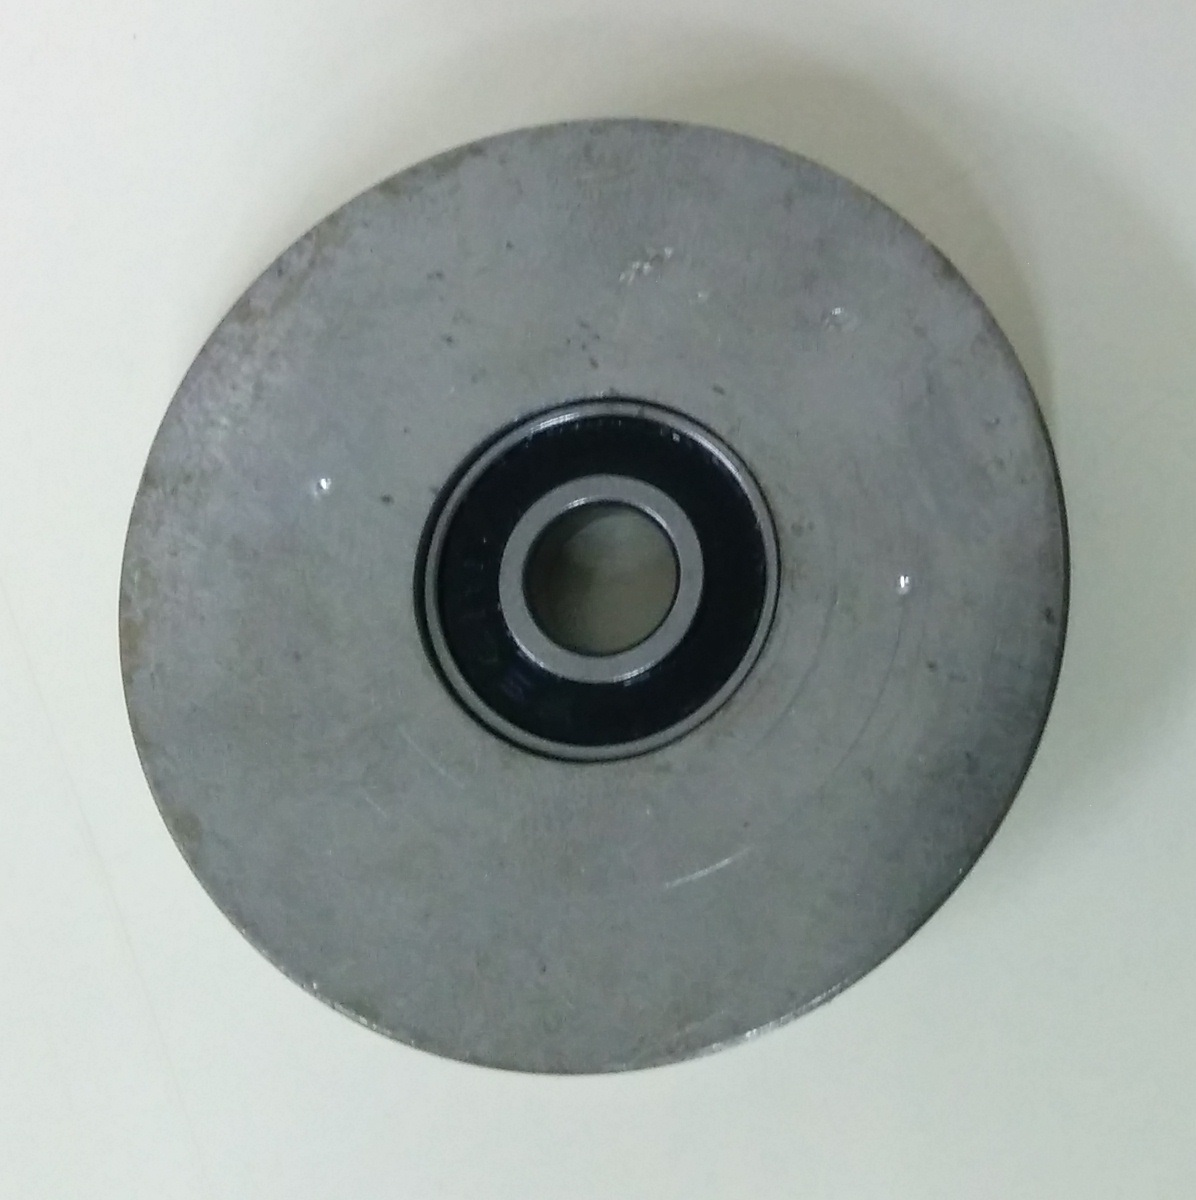
\includegraphics[width=0.8\textwidth]{perlita_rolamento}
		\caption{Amostras de perlita com rolamento.}
		\label{fig:perlita_rolamento}
	\end{figure}
\end{columns}
\end{frame}

\begin{frame}
\frametitle{Preparação das rodas bainíticas}

	Tratamento térmico de austêmpera
	\begin{enumerate}
		\item Aquecimento do material a 900\textdegree C por 15 min;
		\item Imergir o material em um banho de sais a 380\textdegree C por 5 min;
		\item Resfriar sob temperatura ambiente.
		
	\end{enumerate}


	\begin{table}[H]
		\centering
		\caption{Parâmetros utilizados na austêmpera.}
		\resizebox{0.7\textwidth}{!}{%
		\begin{tabular}{|cc|}
			\hline
			\multicolumn{2}{|c|}{Austêmpera} \bigstrut\\
			\hline
			Temperatura de aquecimento & 900$^\circ$C \bigstrut[t]\\
			Tempo de aquecimento & 15 min \\
			Temperatura do banho & 380$^\circ$C \\
			Tempo de resfriamento & 5 min \\
			Tipo de banho & Nitrato de potássio e nitrito de sódio \bigstrut[b]\\
			\hline
		\end{tabular}%
	}
		\label{tab:parametros_austempera}%
	\end{table}%

\end{frame}
	
\begin{frame}
%\frametitle{Preparação das rodas bainíticas}
\begin{figure}
	\centering
	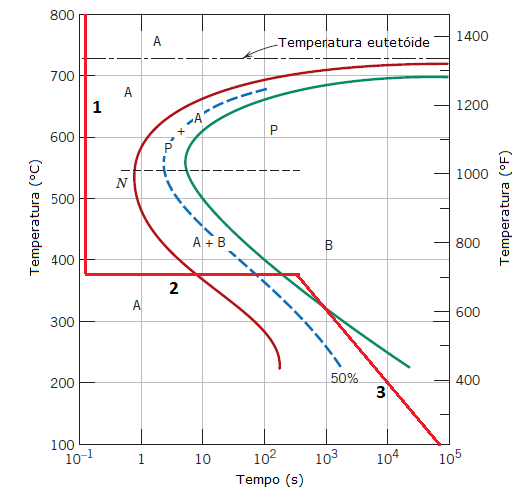
\includegraphics[height=0.8\textheight]{austempera}
	\caption{Diagrama TTT do aço eutetóide com representação da austêmpera.}
	\label{fig:austempera}
\end{figure}
\end{frame}


\begin{frame}
\frametitle{Preparação das rodas bainíticas}
\begin{columns}[c] % The "c" option specifies centered vertical alignment while the "t" option is used for top vertical alignment
	\column{.5\textwidth} % Left column and width
	\begin{figure}
		\centering
		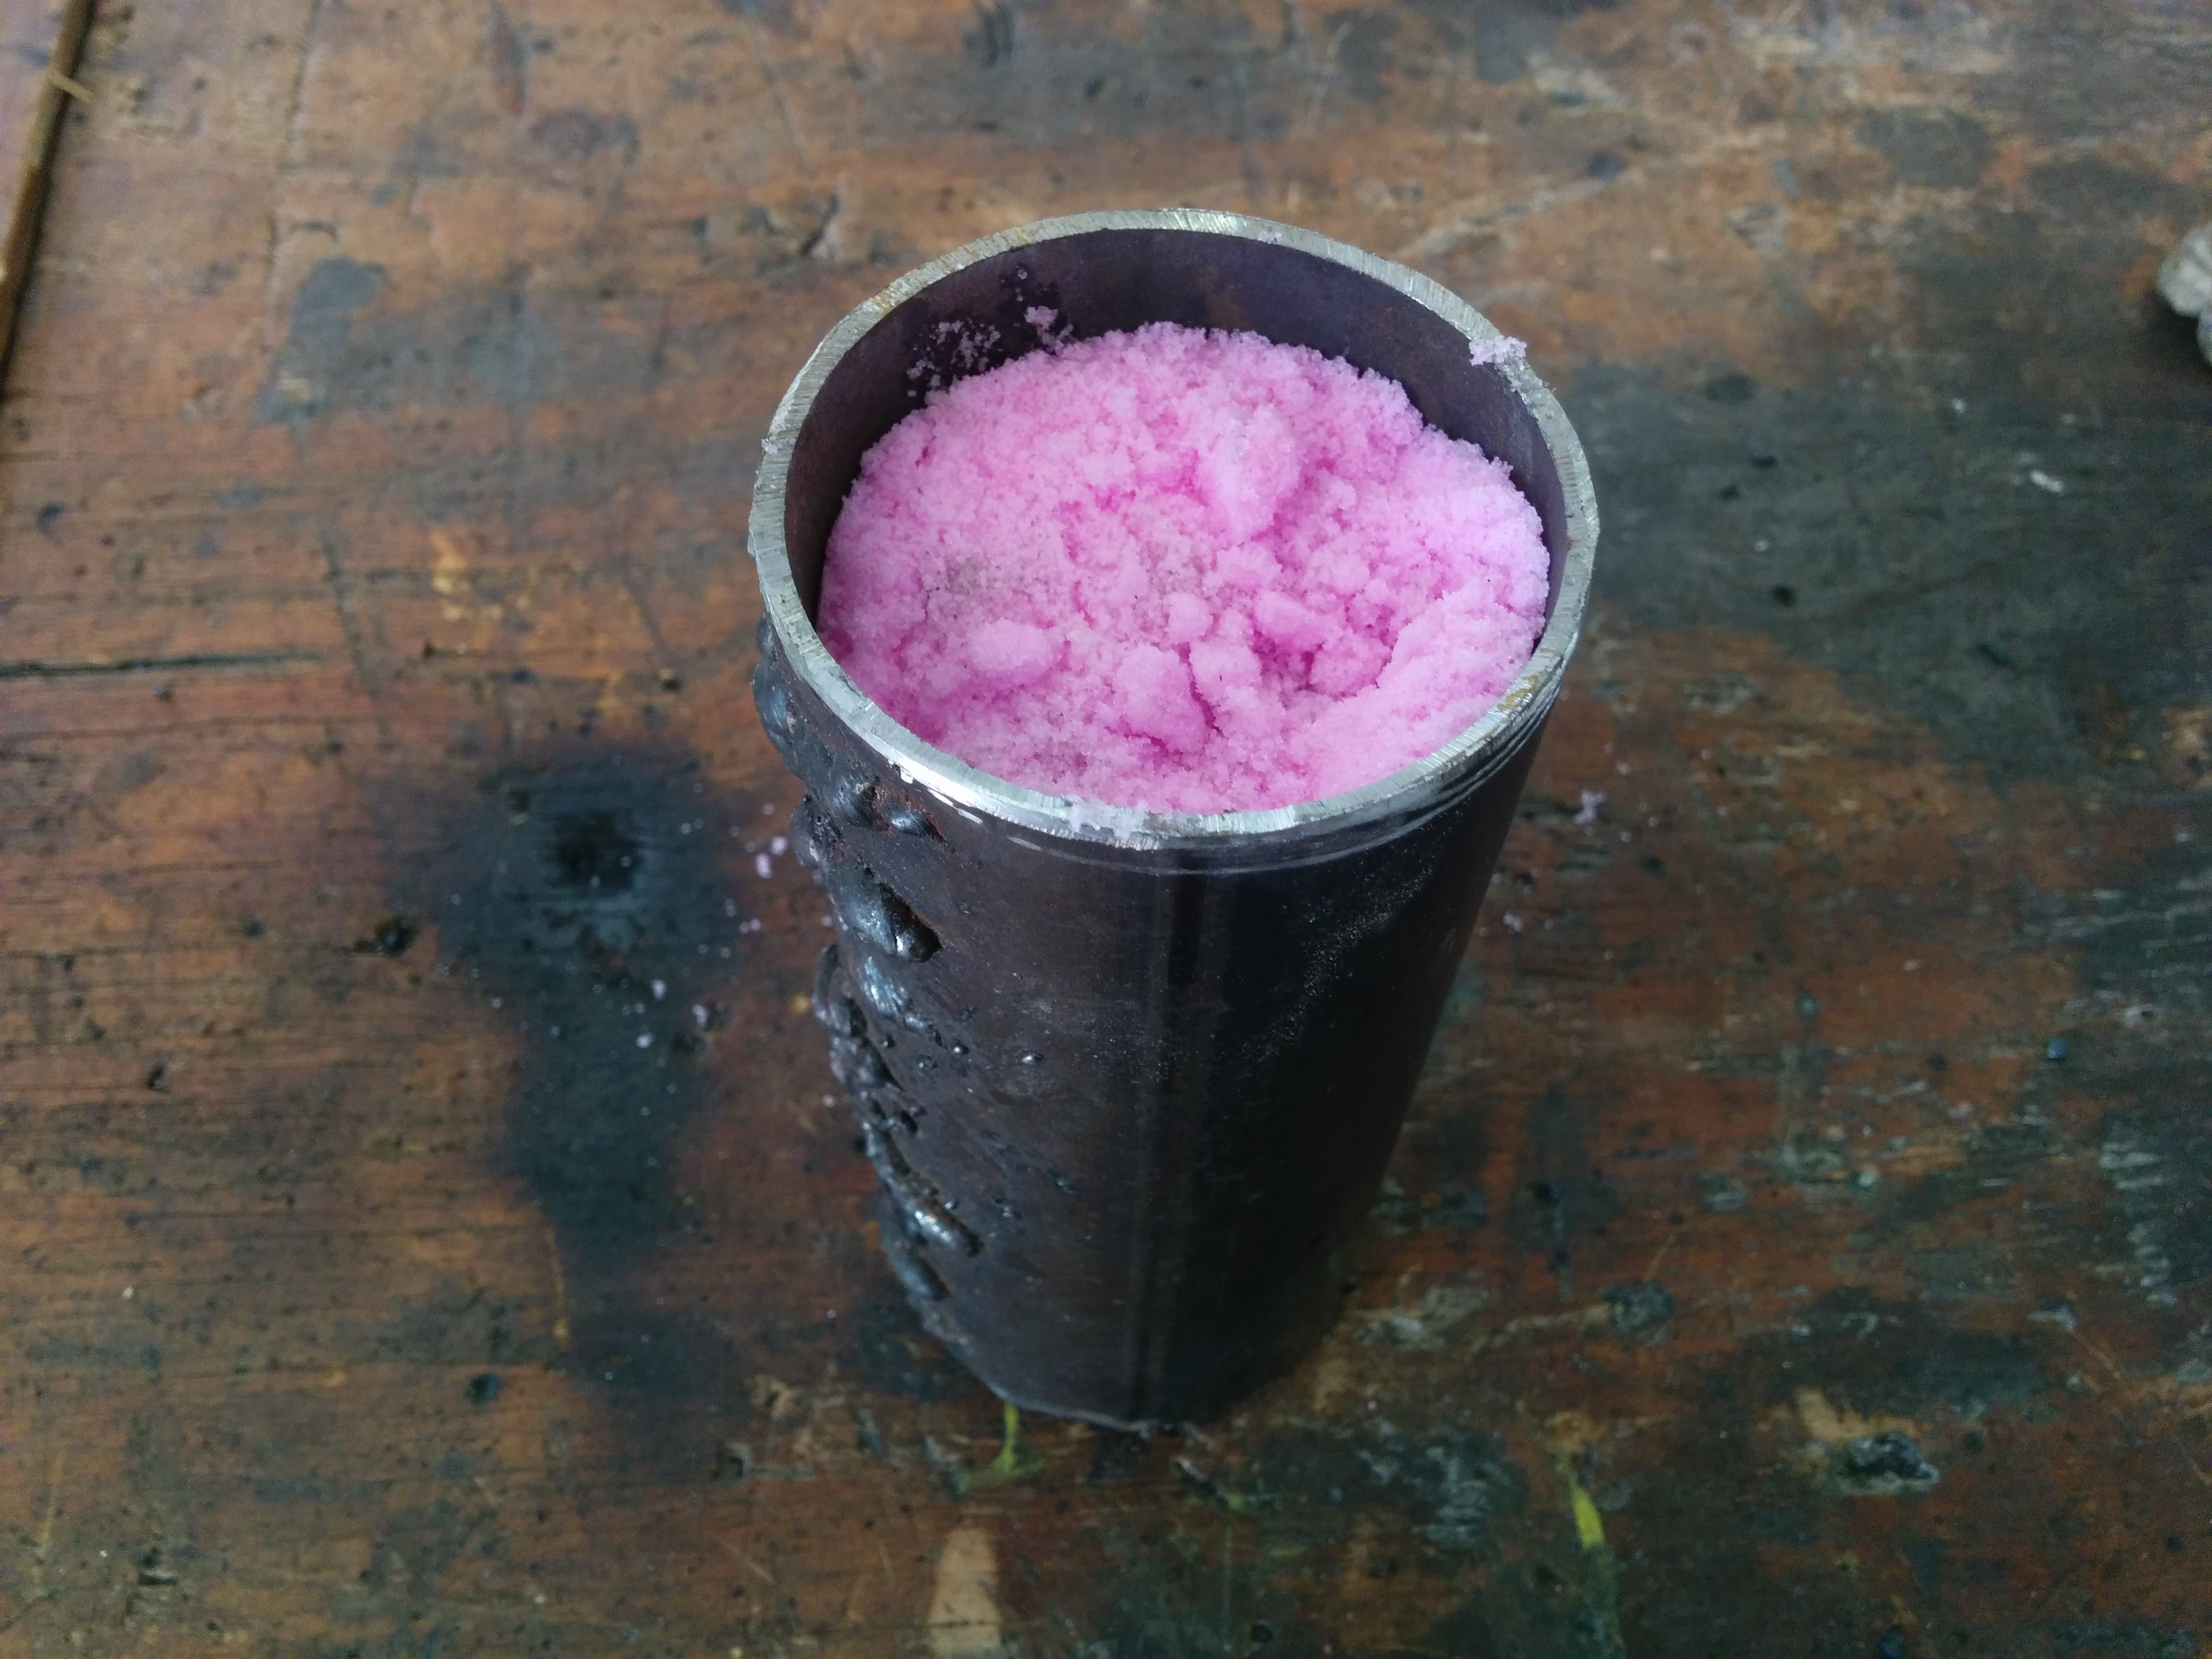
\includegraphics[width=1\textwidth]{sais}
		\caption{Sal utilizado para o banho.}
		\label{fig:sais}
	\end{figure}
	
	\column{.5\textwidth} % Right column and width]
	\begin{figure}
		\centering
		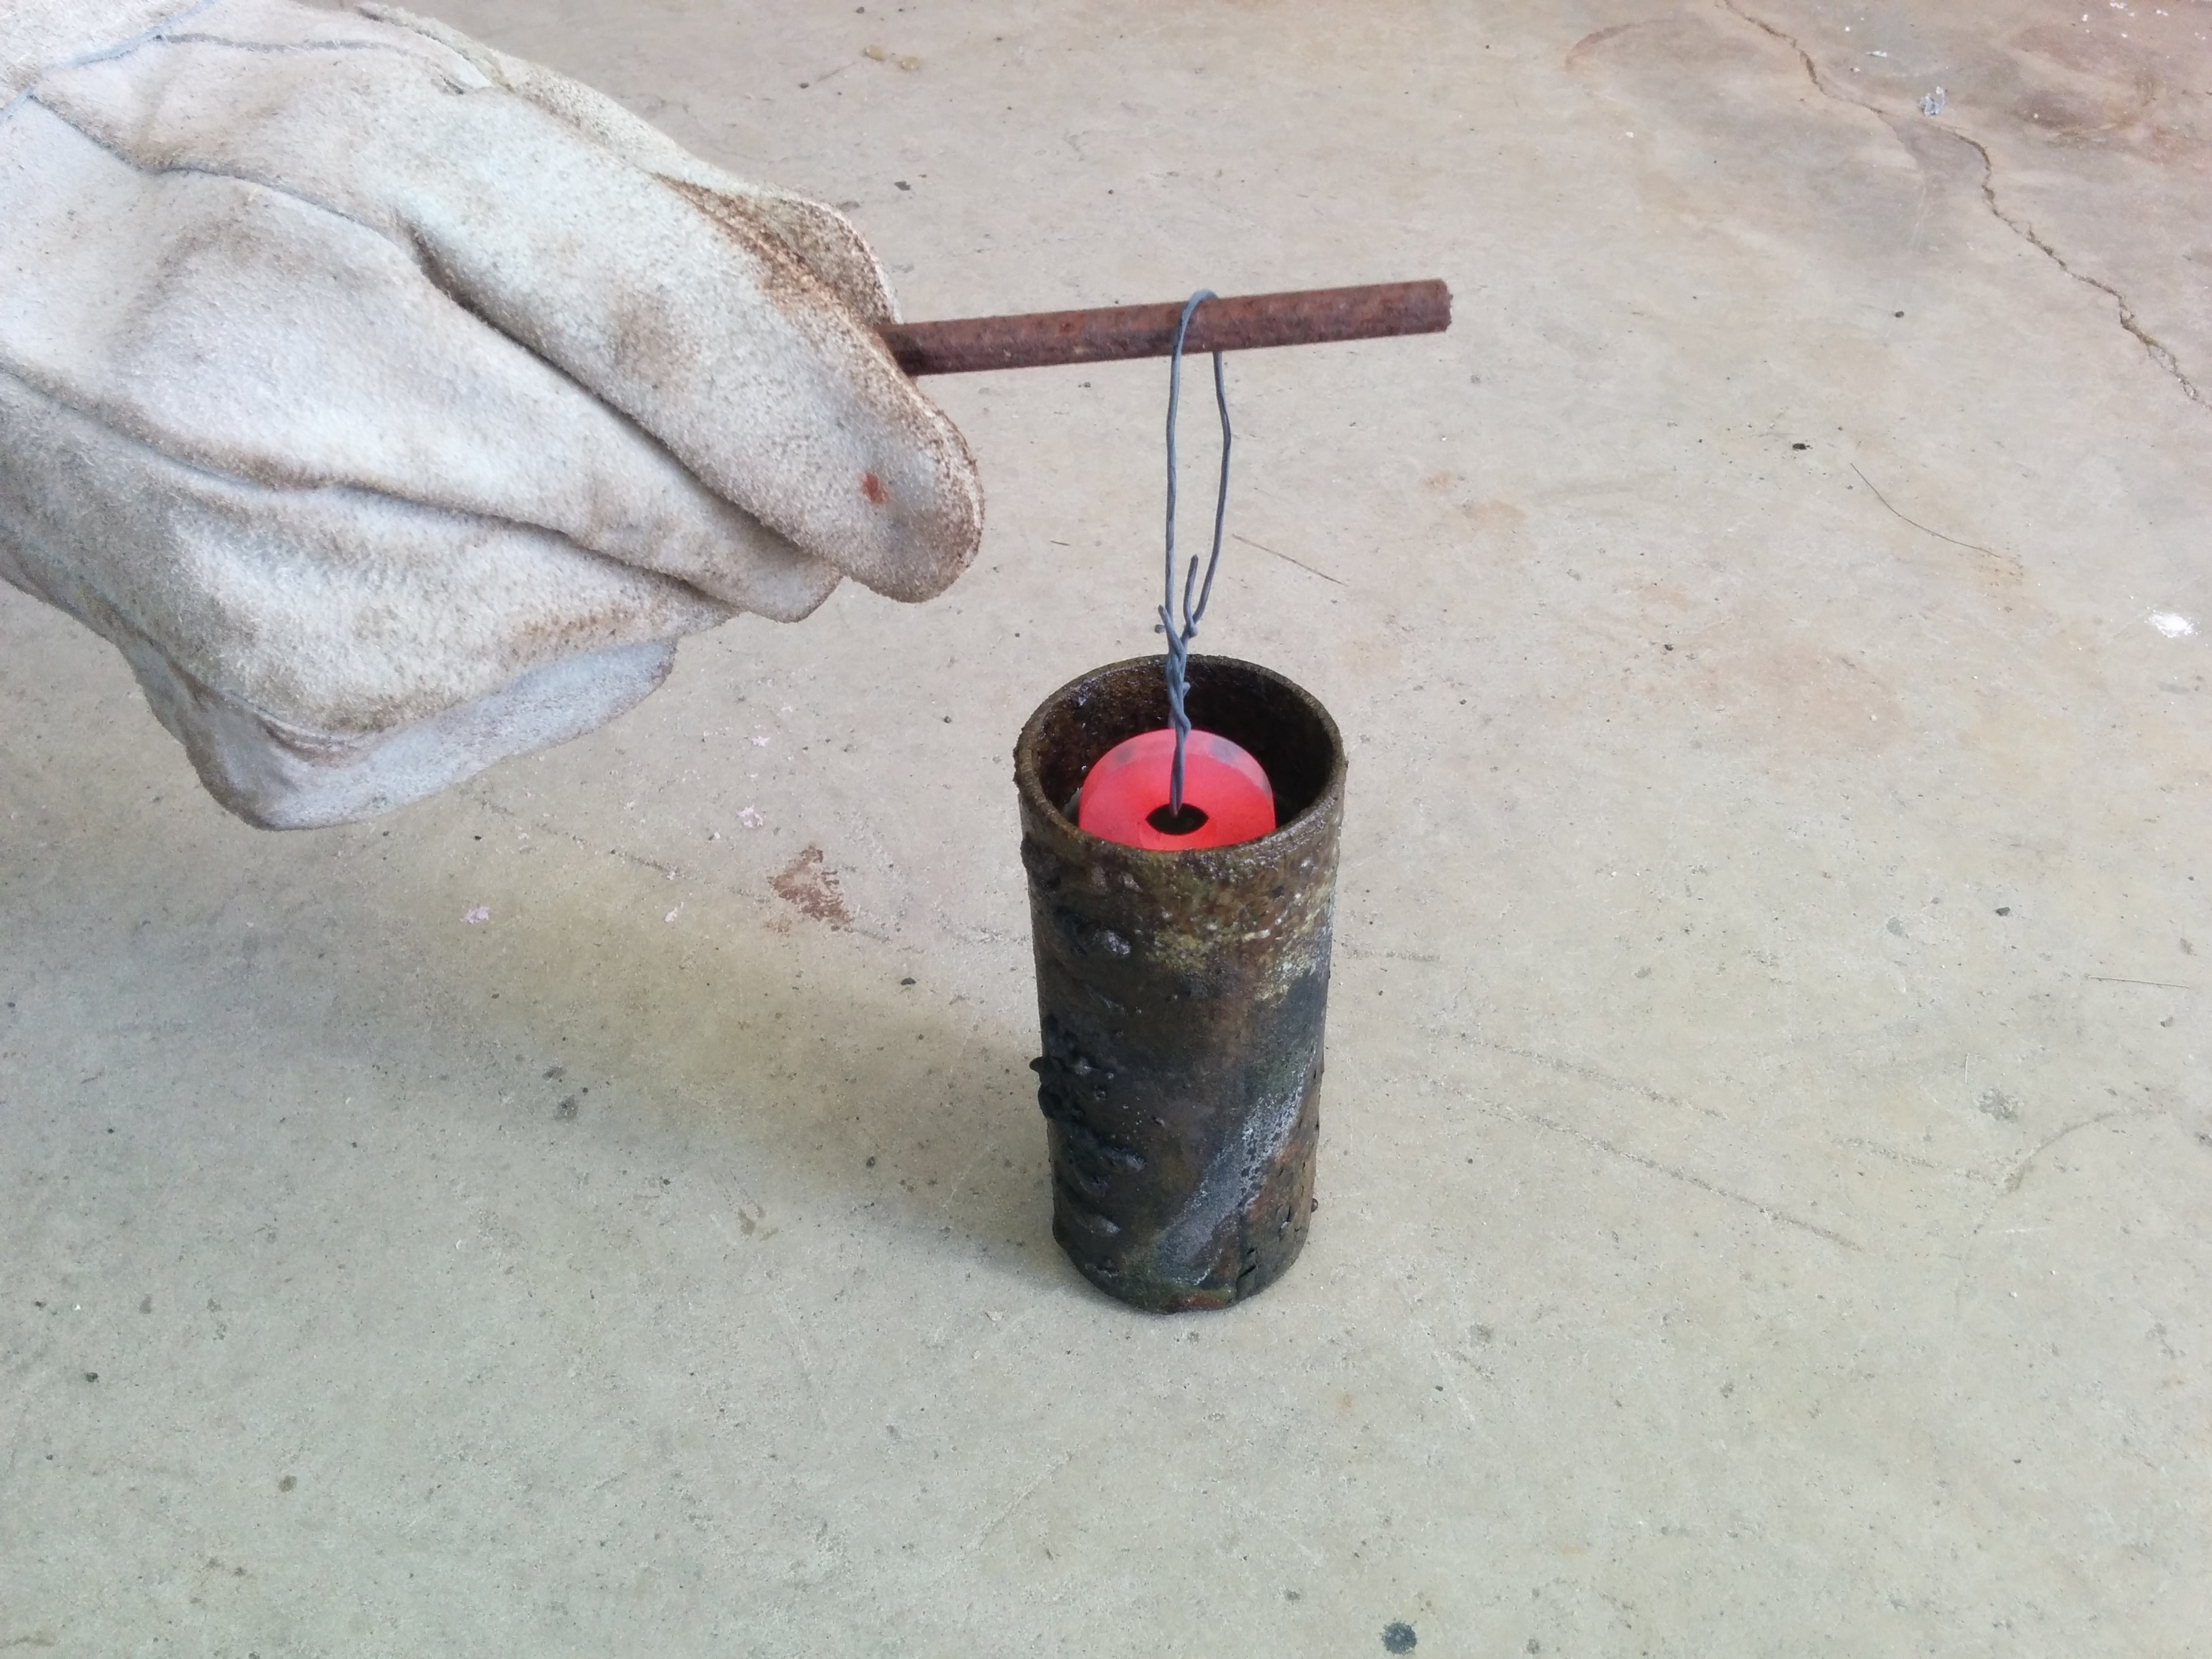
\includegraphics[width=1\textwidth]{resfriamento}
		\caption{Resfriamento da amostra no sal.}
		\label{fig:resfriamento}
	\end{figure}
\end{columns}
\end{frame}

\begin{frame}
\frametitle{Preparação das rodas bainíticas}

\begin{columns}[c] % The "c" option specifies centered vertical alignment while the "t" option is used for top vertical alignment
	\column{.5\textwidth} % Left column and width
	Controle de temperatura:
	\begin{itemize}
		\item Para o sal: através de um pirômetro portátil.
		\item Para a amostra: através do controle de temperatura da mufla
	\end{itemize}
	
	\column{0.5\textwidth} % Right column and width]
	\begin{figure}
		\centering
		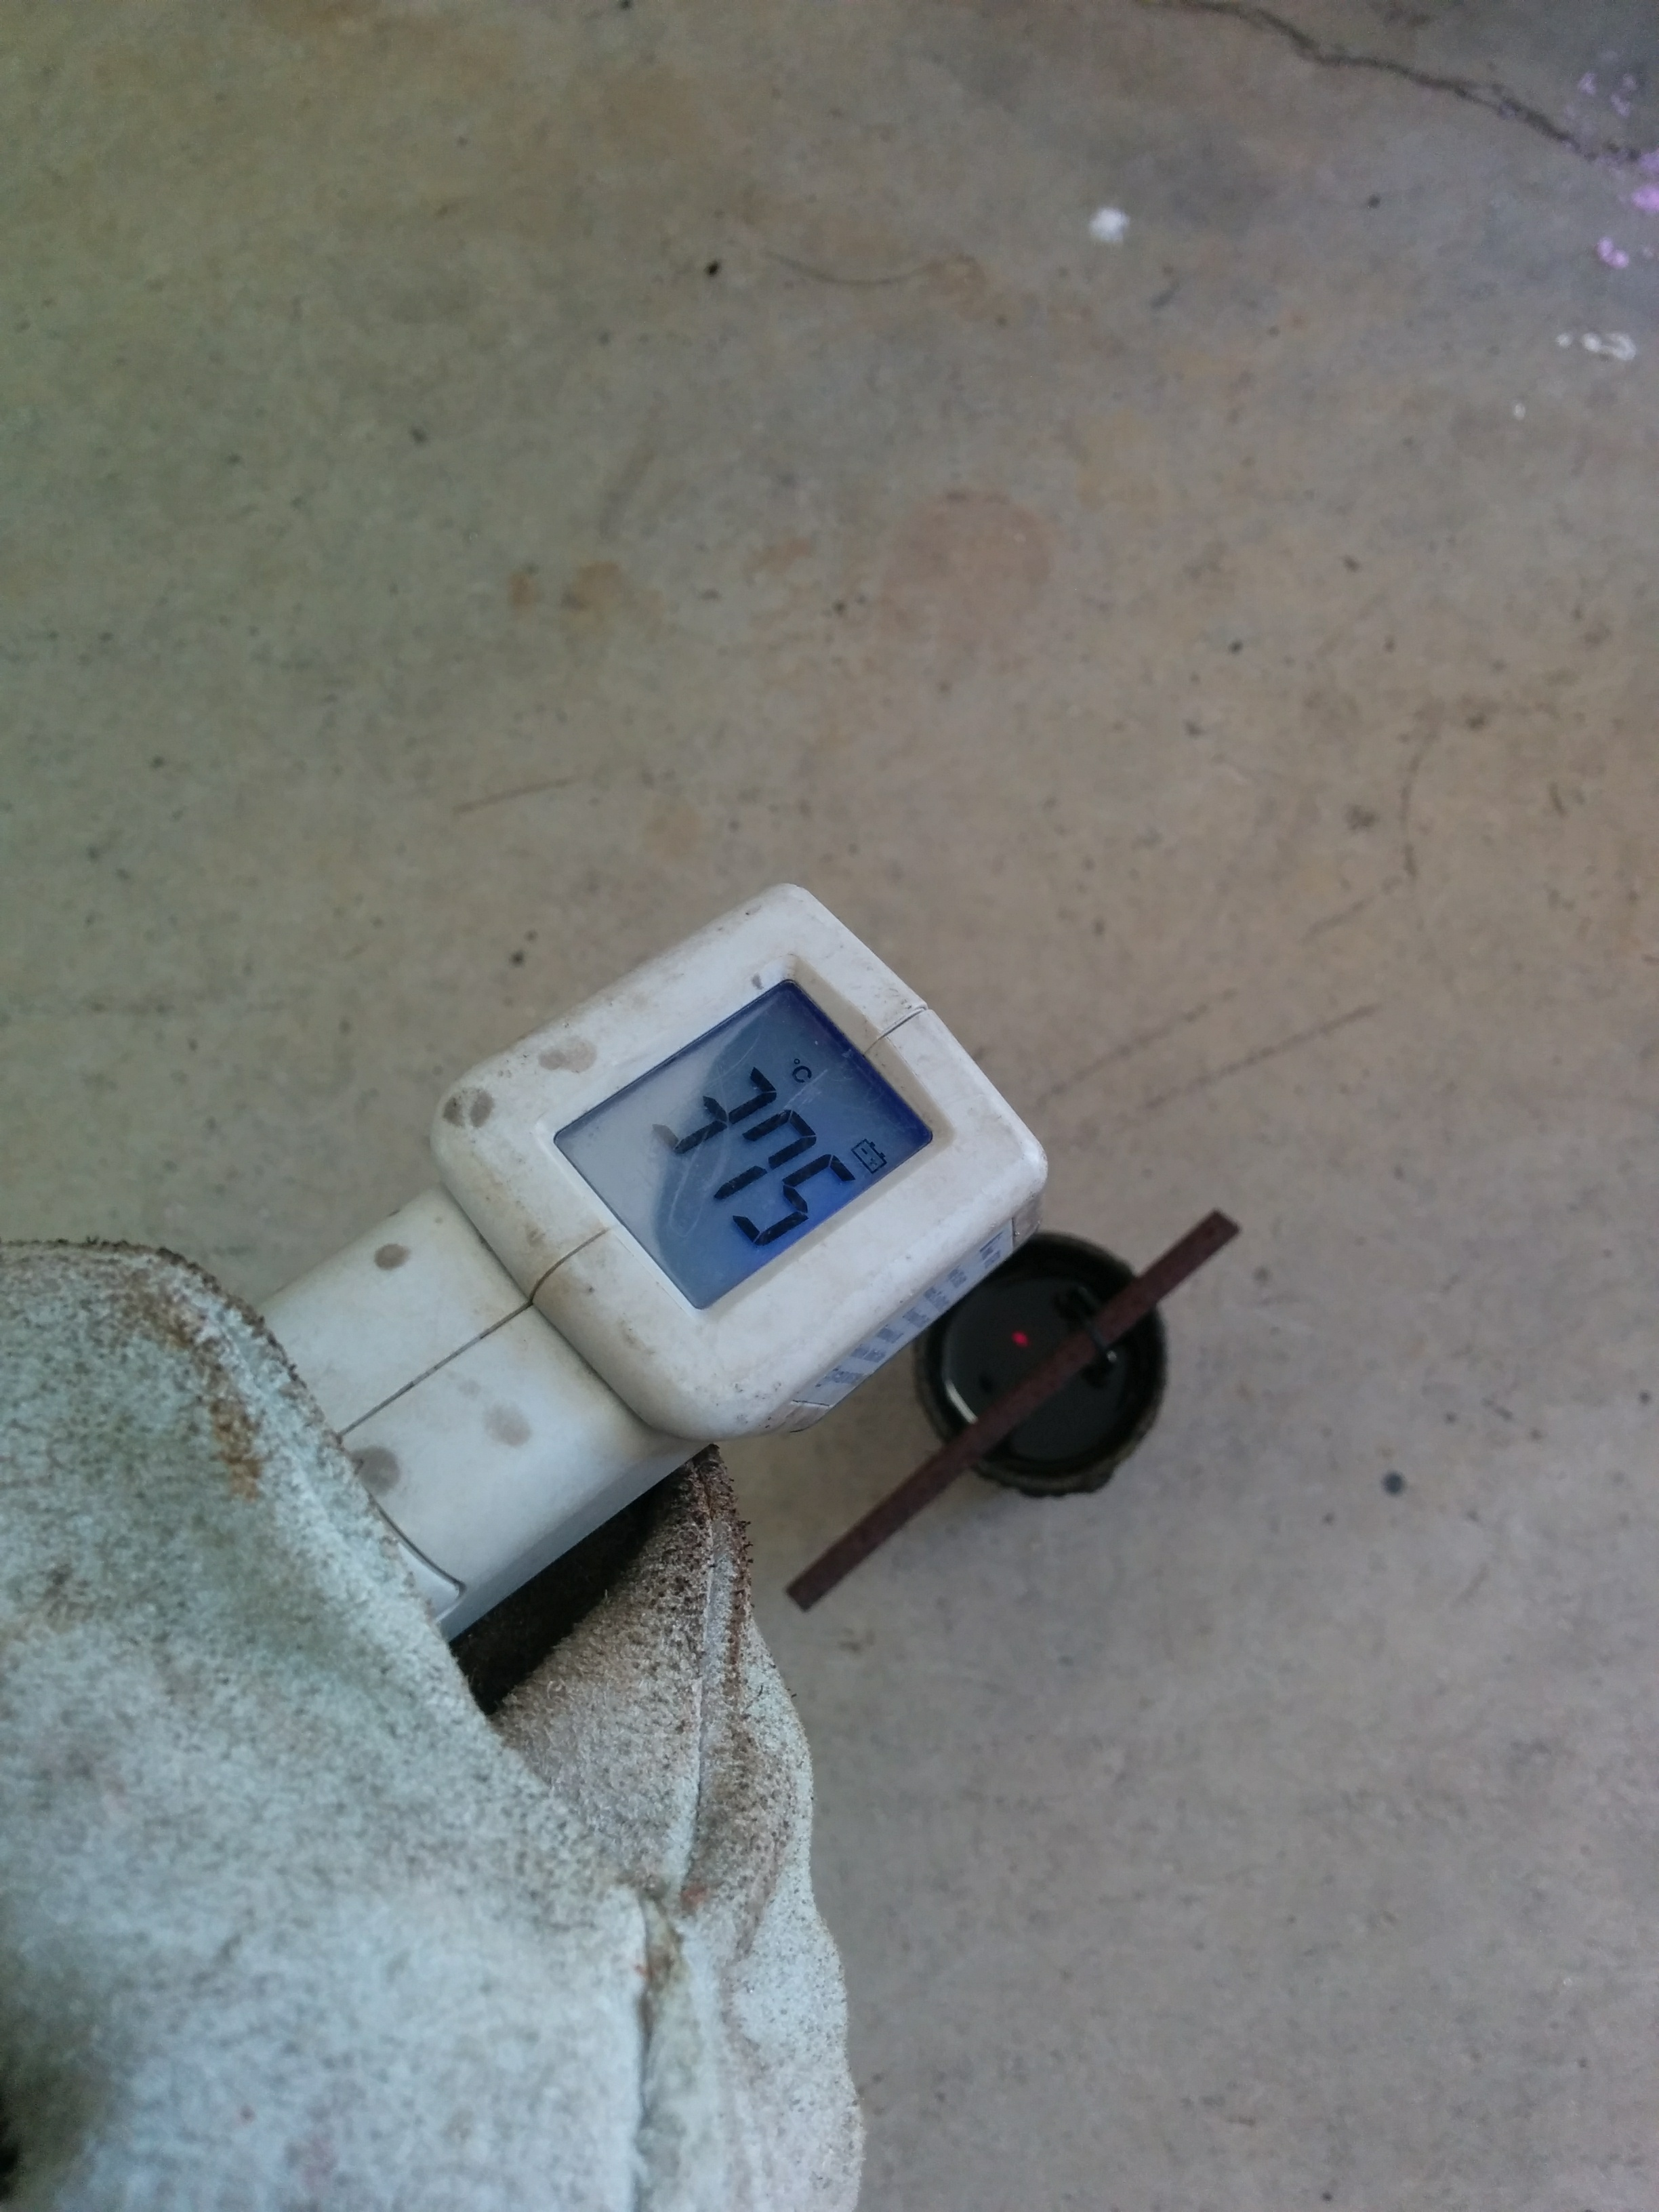
\includegraphics[width=0.7\textwidth]{pirometro}
		\caption{Pirômetro utilizado.}
		\label{fig:pirometro}
	\end{figure}
\end{columns}
\end{frame}

\begin{frame}
\frametitle{Preparação das rodas bainíticas}

\begin{columns}[c] % The "c" option specifies centered vertical alignment while the "t" option is used for top vertical alignment
	\column{.5\textwidth} % Left column and width
	Após o tratamento as amostras foram usinadas da mesma forma que as amostras perlíticas:
	\begin{itemize}
		\item 42 mm de diâmetro e 6 mm de espessura.
		\item Chanfros reduzindo a área de contato para 2 mm.
	\end{itemize}
	
	\column{0.5\textwidth} % Right column and width]
	\begin{figure}
		\centering
		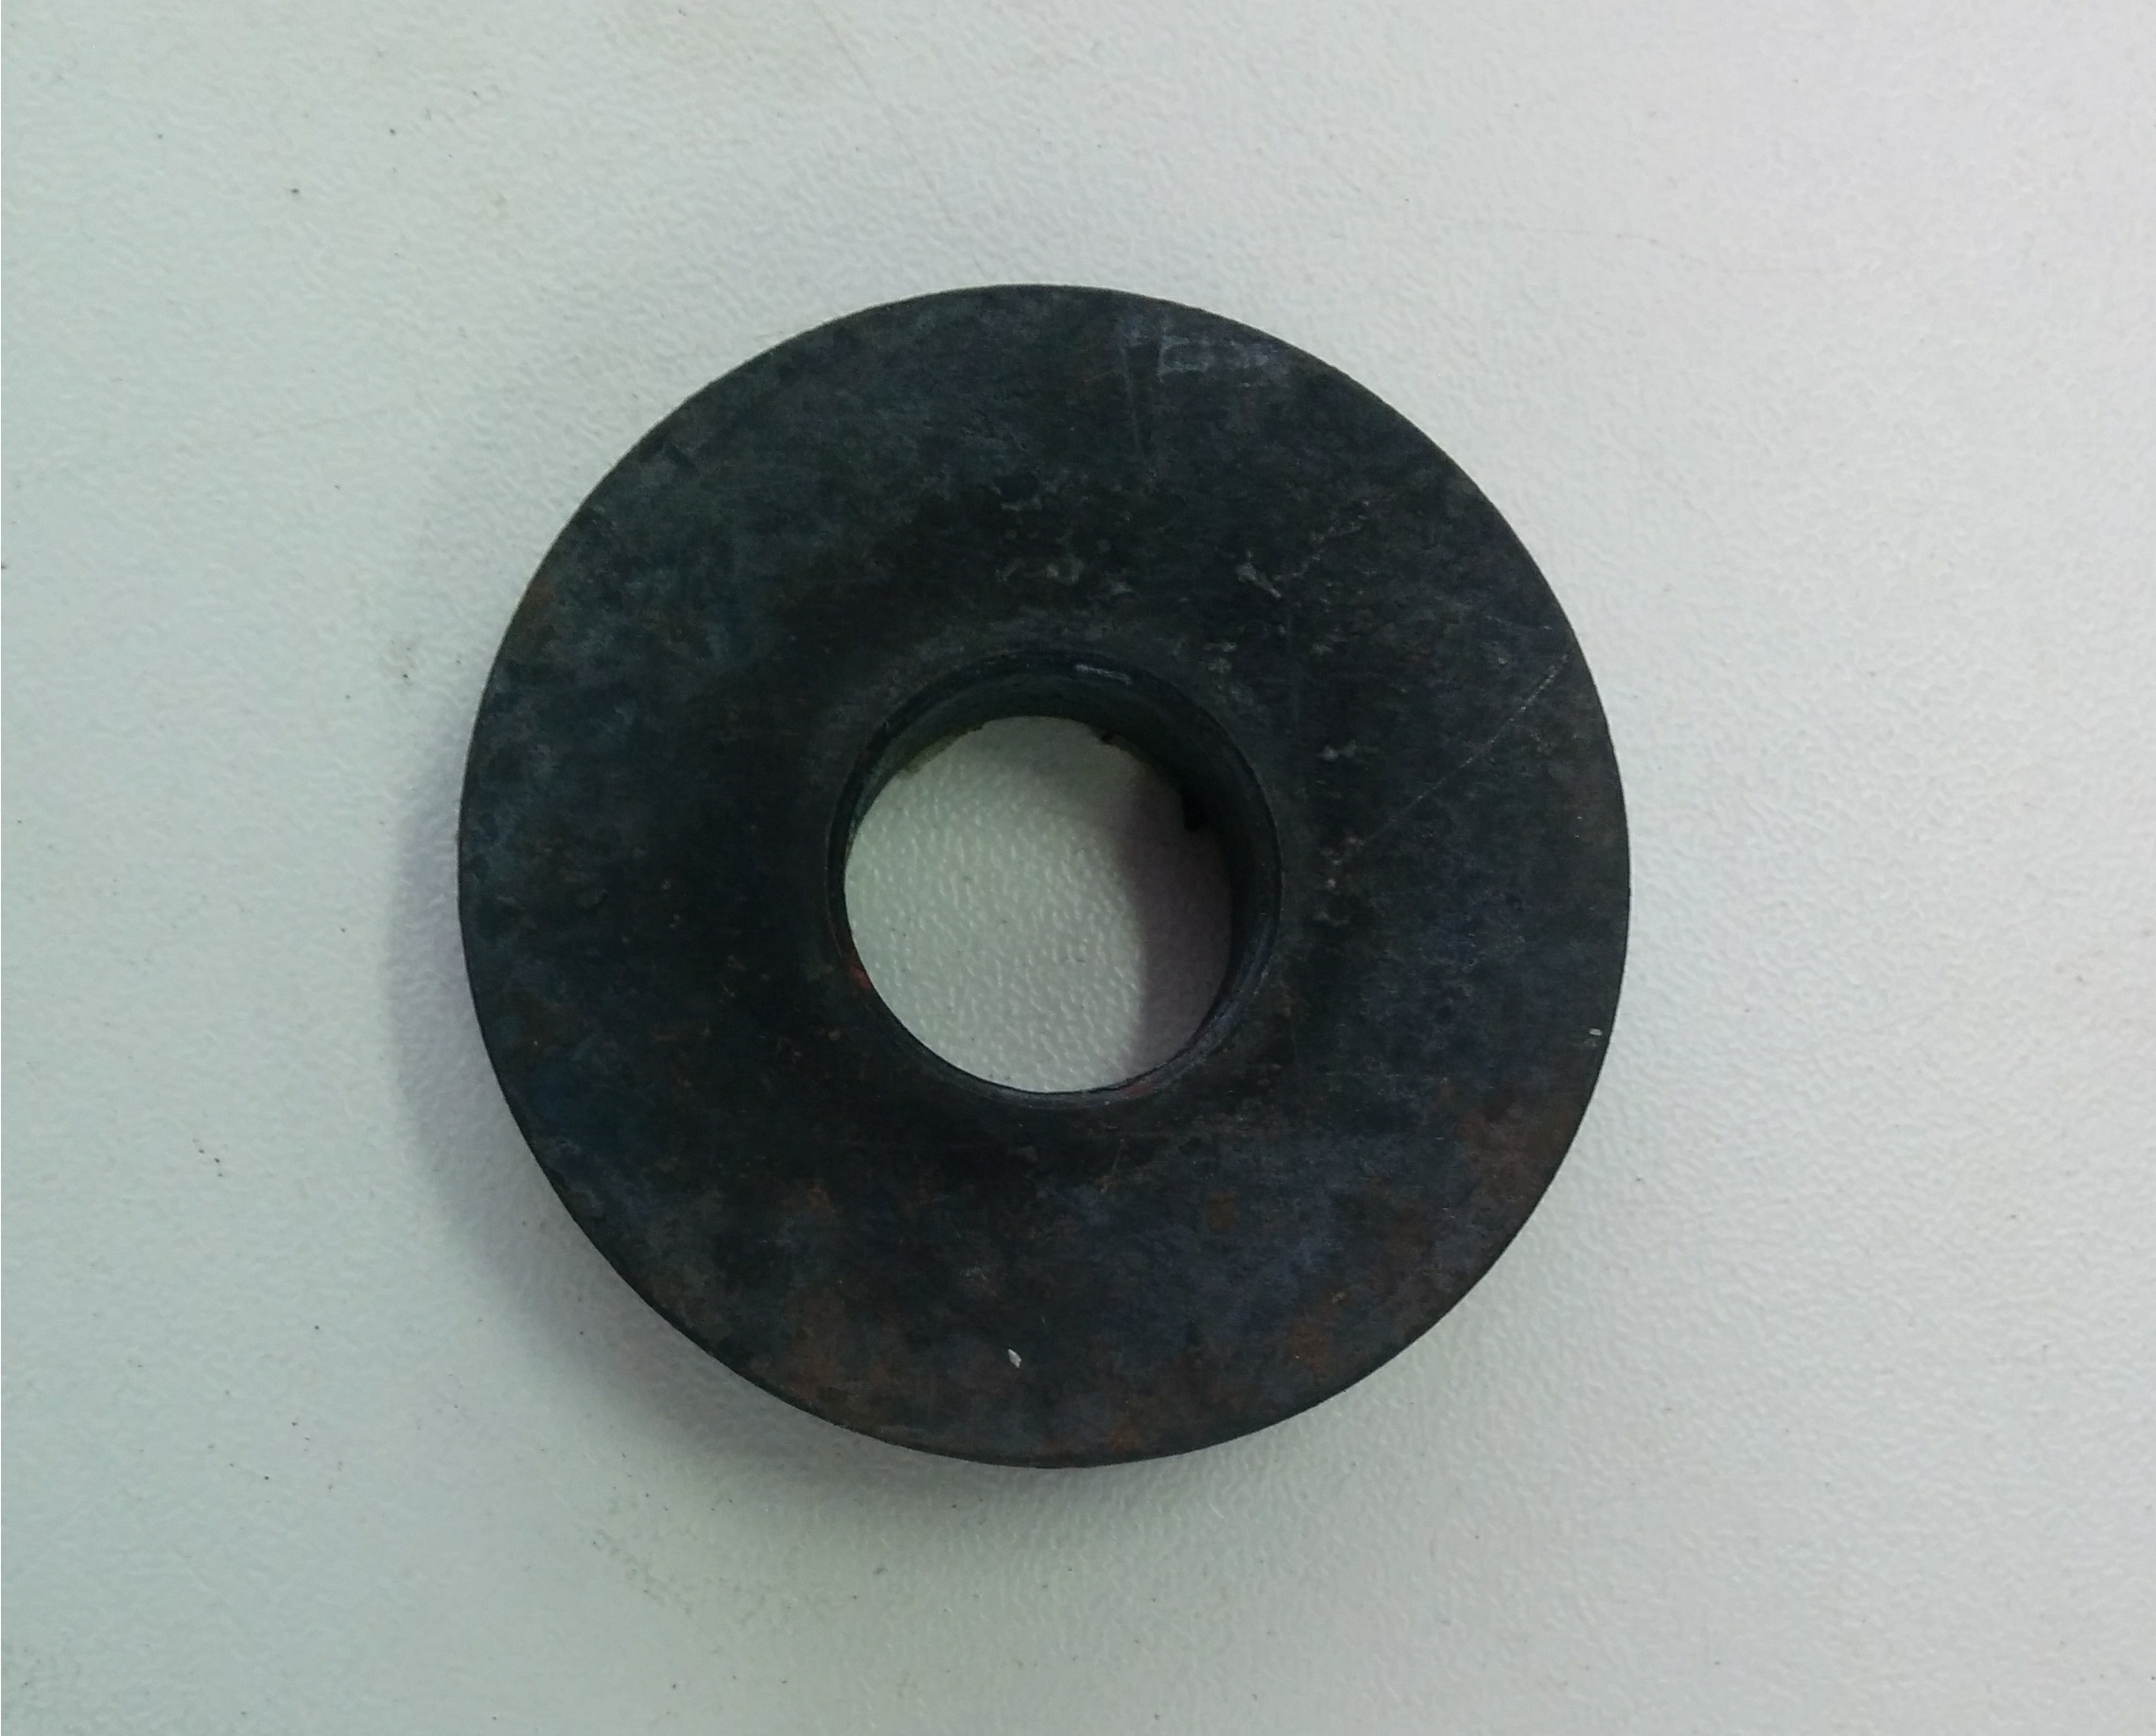
\includegraphics[width=0.7\textwidth]{amostra_bainita}
		\caption{Amostra de bainita após o tratamento térmico.}
		\label{fig:amostra_bainita}
	\end{figure}
\end{columns}

	

\end{frame}



\subsection{Análise de dureza}

\begin{frame}
\frametitle{Dureza pós-austêmpera}

\begin{table}[H]
	\centering
	\caption{Leituras obtidas para as amostras perlíticas e para as amostras bainíticas (pós tratamento de austêmpera).}
	\resizebox{0.6\textwidth}{!}{%
	\begin{tabular}{|ccc|ccc|}
		\hline
		\multicolumn{6}{|c|}{Dureza (HRC)} \bigstrut\\
		\hline
		Amostra    & Leitura    & Média      & Amostra    & Leitura    & Média \bigstrut\\
		\hline
		\multirow{3}[2]{*}{Perlita 1} & 40         & \multirow{3}[2]{*}{40,3} & \multirow{3}[2]{*}{Bainita 1} & 59         & \multirow{3}[2]{*}{59,7} \bigstrut[t]\\
		& 40         &            &            & 60         &  \\
		& 41         &            &            & 60         &  \bigstrut[b]\\
		\hline
		\multirow{3}[2]{*}{Perlita 2} & 40         & \multirow{3}[2]{*}{40,3} & \multirow{3}[2]{*}{Bainita 2} & 42         & \multirow{3}[2]{*}{44,0} \bigstrut[t]\\
		& 40         &            &            & 45         &  \\
		& 41         &            &            & 45         &  \bigstrut[b]\\
		\hline
		\multirow{3}[2]{*}{Perlita 3} & 41         & \multirow{3}[2]{*}{40,7} & \multirow{3}[2]{*}{Bainita 3} & 56         & \multirow{3}[2]{*}{53,7} \bigstrut[t]\\
		& 41         &            &            & 52         &  \\
		& 40         &            &            & 53         &  \bigstrut[b]\\
		\hline
	\end{tabular}%
}
	\label{tab:dureza_pos_austempera}%
\end{table}%

\end{frame}

\begin{frame}
\frametitle{Dureza pós-austêmpera}

\begin{itemize}
	\item O tratamento de austêmpera elevou consideravelmente a dureza dessas amostras bainíticas
	\item Sem uma dureza comum, não é possível comparar dois materiais em desgaste, conforme a Equação de Archard
\end{itemize}

\begin{equation}
Q = K\frac{W}{H}
\end{equation}


\end{frame}

\begin{frame}
\frametitle{Revenido}
\begin{itemize}
	\item Realizou-se o processo de revenimento nos corpos de prova que foram austemperados, que se consiste em reaquecer o corpo de prova a uma temperatura muito inferior à da fase de austenitização e manter sob tal temperatura por um intervalo de tempo.
	\item Os materiais permaneceram no forno por 20 min e, logo em seguida, foram resfriados com
	água, para evitar a fragilização no revenido.
\end{itemize}
\end{frame}

\begin{frame}
\frametitle{Revenido}

\begin{figure}
	\centering
	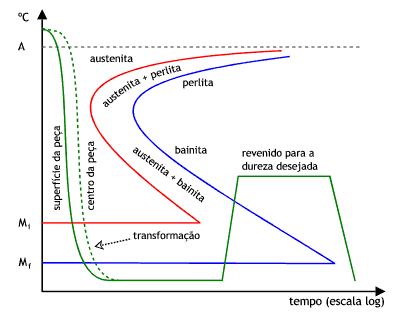
\includegraphics[width=0.6\textwidth]{revenid}
	\caption{Diagrama TTT representando o processo de revenimento das amostras bainíticas.}
	\label{fig:revenid}
\end{figure}

\end{frame}

\begin{frame}
\frametitle{Dureza pós-revenido}

	% Table generated by Excel2LaTeX from sheet 'Sheet1'
\begin{table}[H]
	\centering
	\caption{Valores de dureza obtidos para as amostras perlíticas, bainíticas pós-revenimento e para o contracorpo.}
	\resizebox{0.7\textwidth}{!}{%
		\begin{tabular}{|ccc|ccc|ccc|}
			\hline
			\multicolumn{9}{|c|}{Dureza (HRC)} \bigstrut\\
			\hline
			Amostra & Leitura & Média & Amostra & Leitura & Média & Amostra & Leitura & Média \bigstrut\\
			\hline
			\multirow{4}[2]{*}{Perlita 1} & 40,0 & \multirow{4}[2]{*}{39,9} & \multirow{4}[2]{*}{Bainita 1} & 38,5 & \multirow{4}[2]{*}{40,5} & \multicolumn{1}{c}{\multirow{12}[6]{*}{Contracorpo}} & \multirow{3}[1]{*}{43,5} & \multirow{12}[6]{*}{41,3} \bigstrut[t]\\
			& 41,0 &   &   & 41,0 &   &   &   &  \\
			& 39,0 &   &   & 41,0 &   &   &   &  \\
			& 39,5 &   &   & 41,5 &   &   & \multirow{3}[2]{*}{40,0} &  \bigstrut[b]\\
			\cline{1-6}    \multirow{4}[2]{*}{Perlita 2} & 38,0 & \multirow{4}[2]{*}{39,6} & \multirow{4}[2]{*}{Bainita 2} & 38,0 & \multirow{4}[2]{*}{36,9} &   &   &  \bigstrut[t]\\
			& 39,0 &   &   & 37,0 &   &   &   &  \\
			& 40,0 &   &   & 36,5 &   &   & \multirow{3}[2]{*}{41,5} &  \\
			& 41,5 &   &   & 36,0 &   &   &   &  \bigstrut[b]\\
			\cline{1-6}    \multirow{4}[2]{*}{Perlita 3} & 40,5 & \multirow{4}[2]{*}{40,6} & \multirow{4}[2]{*}{Bainita 3} & 40,0 & \multirow{4}[2]{*}{40,9} &   &   &  \bigstrut[t]\\
			& 41,0 &   &   & 40,0 &   &   & \multirow{3}[1]{*}{40,0} &  \\
			& 41,0 &   &   & 41,0 &   &   &   &  \\
			& 40,0 &   &   & 42,5 &   &   &   &  \bigstrut[b]\\
			\hline
		\end{tabular}%
	}
	\label{tab:dureza_pos_revenimento}%
\end{table}%

\end{frame}



\subsection{Micrografia}

\begin{frame}
\frametitle{Análise da superfície das amostras}

Objetivos:
\begin{enumerate}
	\item Investigar os detalhes da microestrutura das amostras bainíticas e perlíticas;
	\item Assegurar que o tratamento térmico das amostras bainíticas foi realizado de maneira correta;
	\item Certificar-se que a microestrutura original das amostras é de fato a perlita.
\end{enumerate}


\end{frame}

\begin{frame}
\frametitle{Corte das amostras para micrografia}

\begin{itemize}
	\item Uma das três amostras de cada microestrutura foi cortada para analisar sua superfície.
	\item O corte foi feito estrategicamente para uma obervação da forma e tamanho do grão no centro do corpo de prova.
	\item Foi realizada a microscopia eletrônica de varredura.
\end{itemize}

\begin{figure}
	\centering
	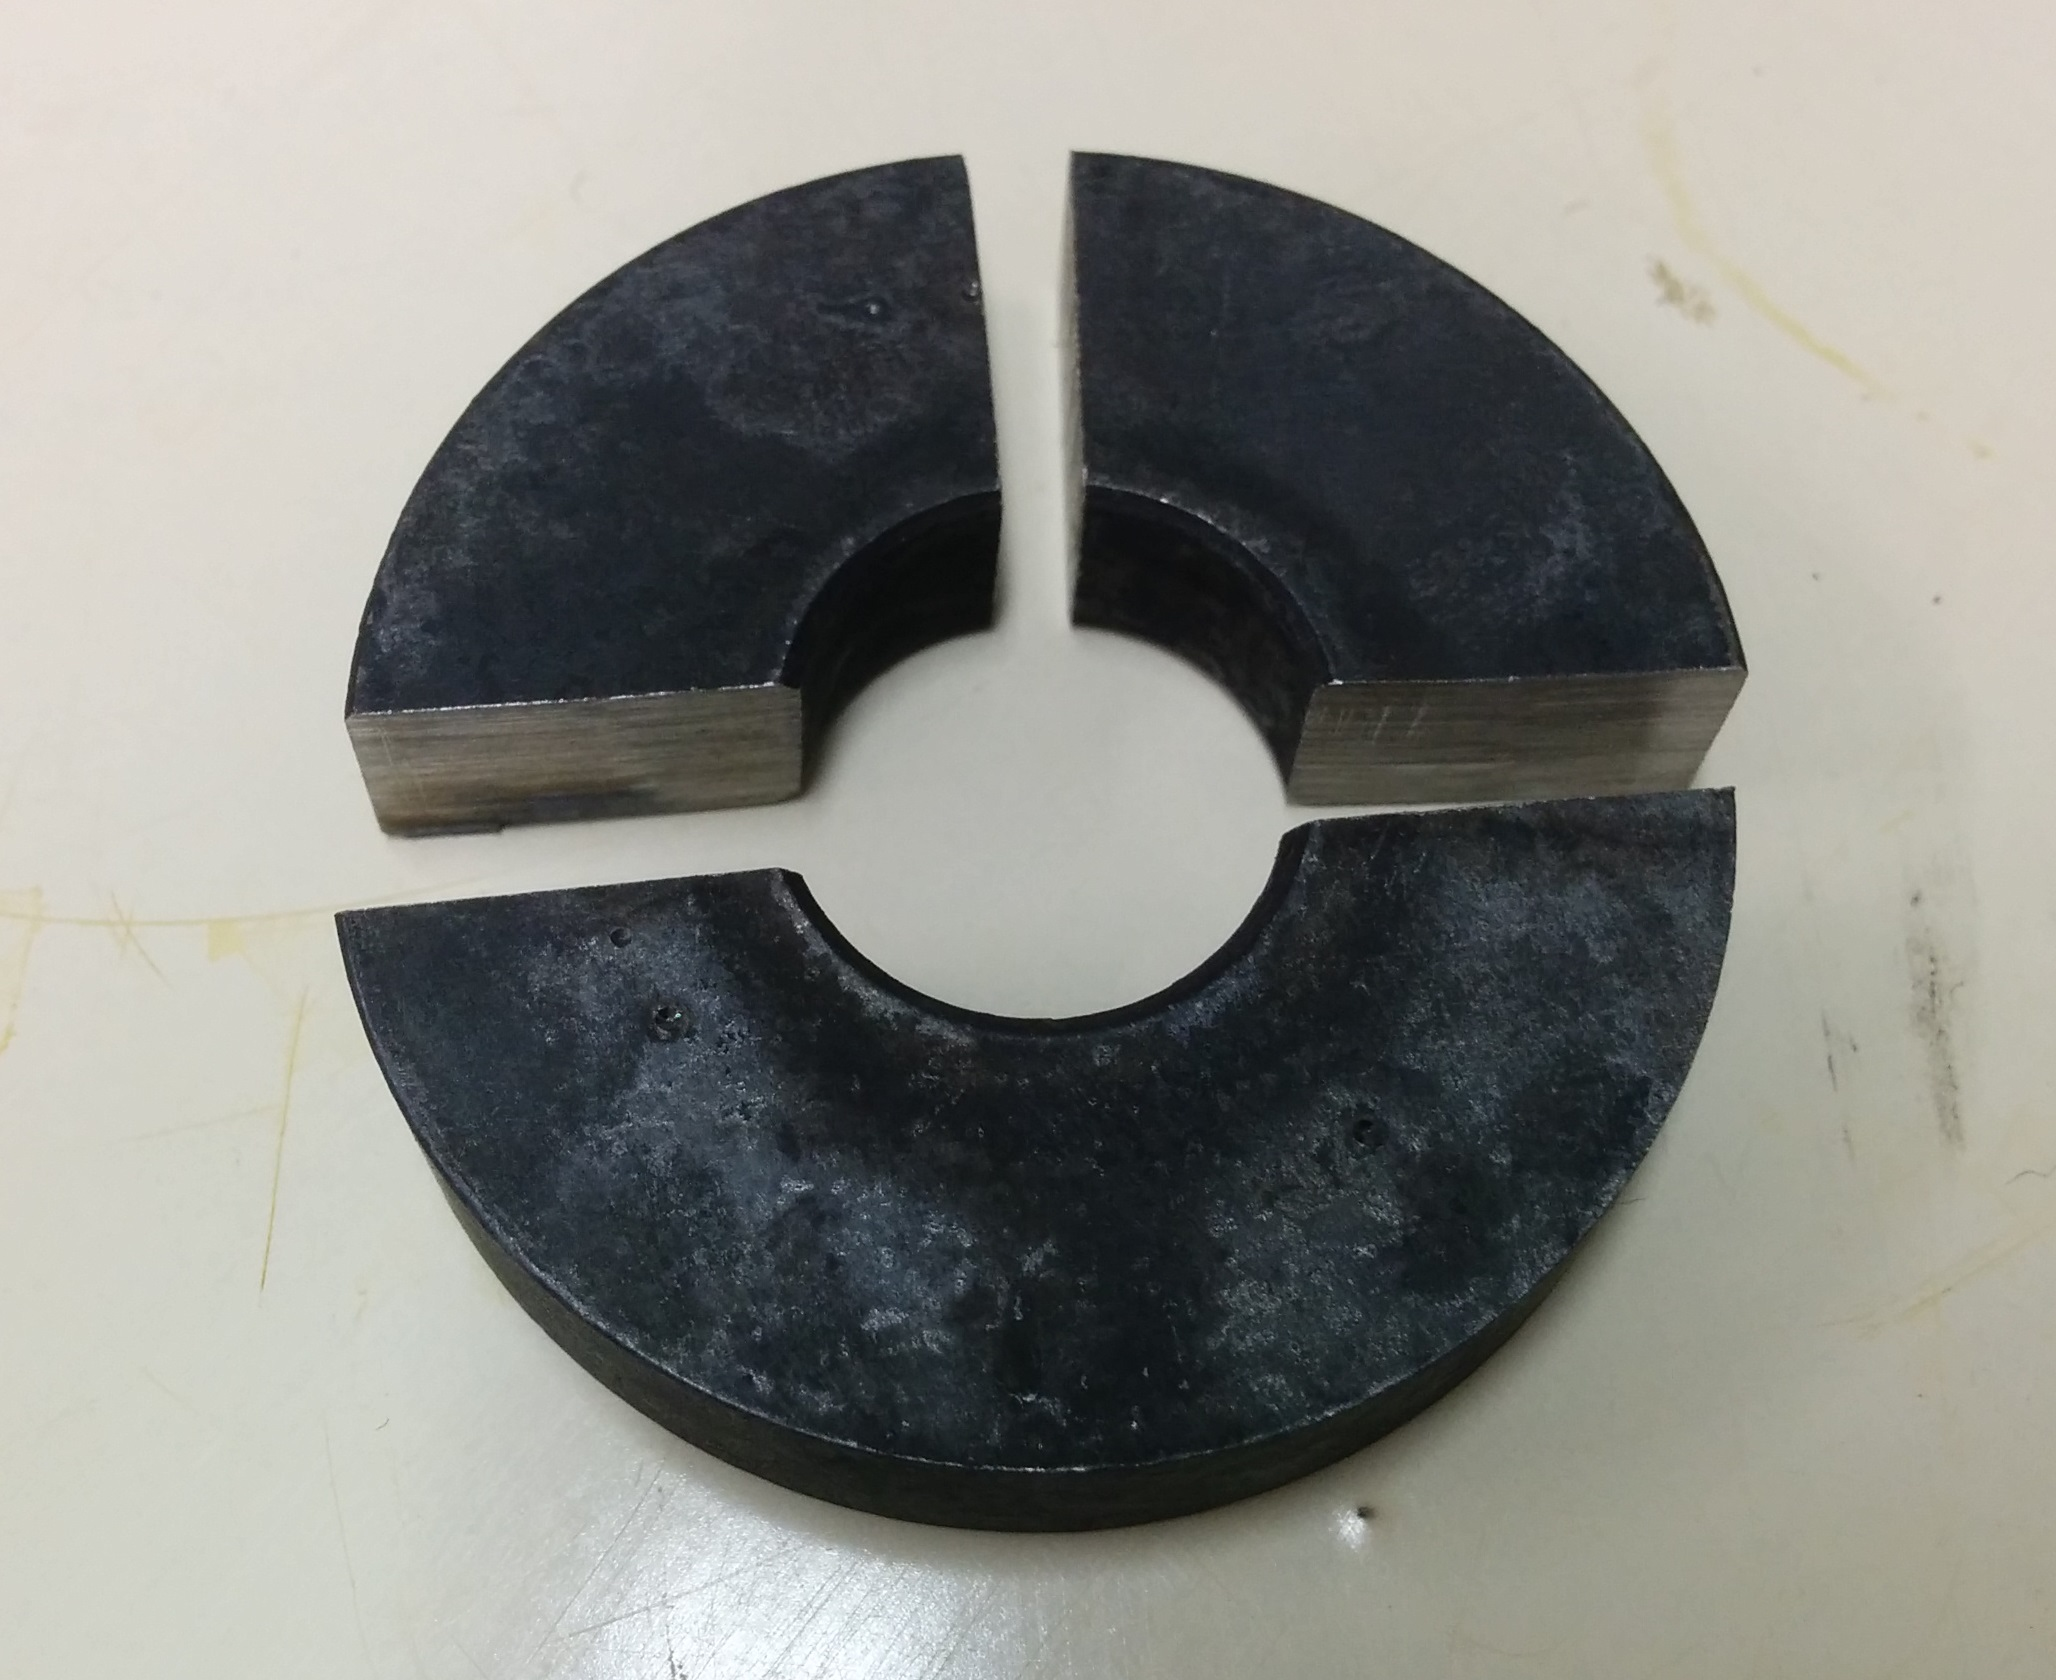
\includegraphics[width=0.3\textwidth]{corte_micrografia}
	\caption{Esquema de corte na amostra perlítica e bainítica para análise.}
	\label{fig:corte_micrografia}
\end{figure}


\end{frame}

\begin{frame}
\frametitle{Micrografia da amostra bainítica}
\begin{figure}
	\centering
	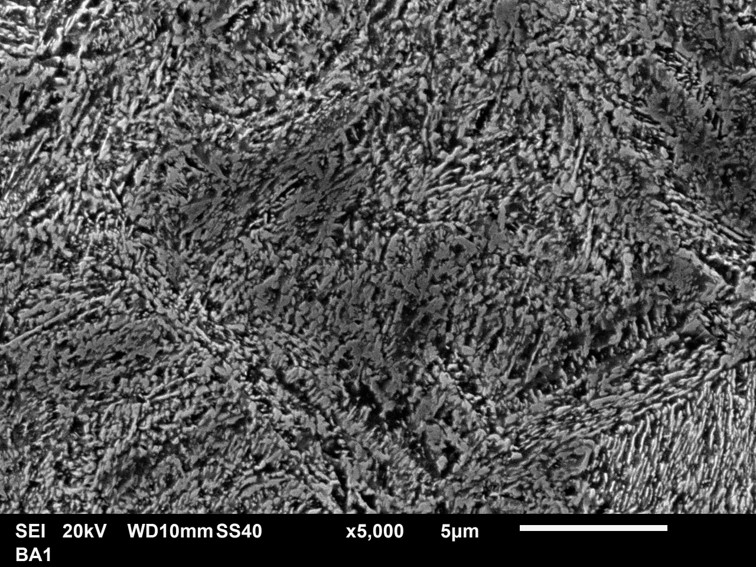
\includegraphics[width=0.65\textwidth]{bainita_top}
	\caption{Micrografia da amostra bainítica com ampliação de 5000x.}
	\label{fig:bainita_top}
\end{figure}
\end{frame}


\begin{frame}
\frametitle{Amostra bainítica - Comparação com a bibliografia}
\begin{figure}
	\centering
	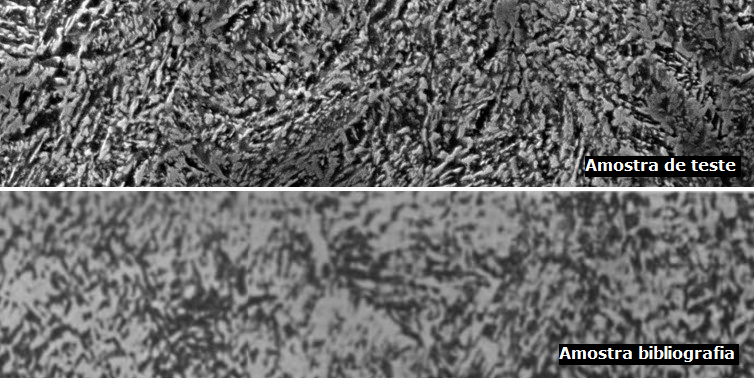
\includegraphics[width=0.85\textwidth]{comparacao_bainita}
	\caption{Comparação entre a micrografia obtida e a bibliografia.}
	\label{fig:comparacao_bainita}
\end{figure}
\end{frame}

\begin{frame}
\frametitle{Micrografia da amostra perlítica}
\begin{figure}
	\centering
	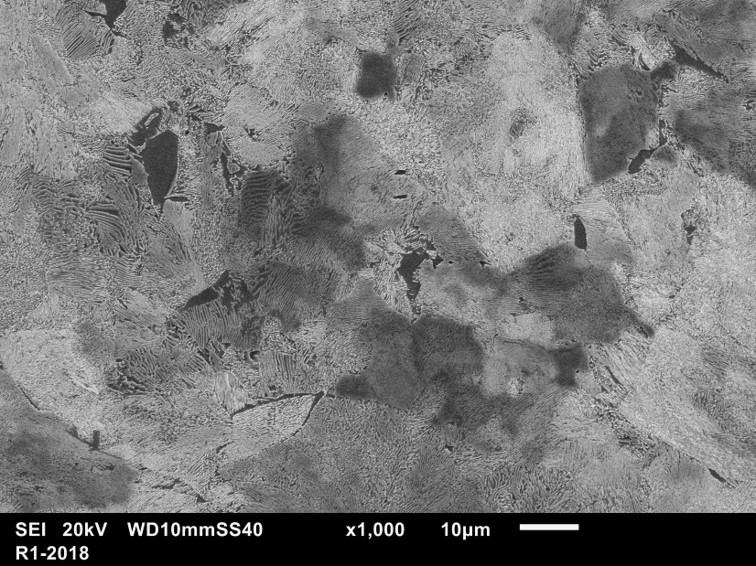
\includegraphics[width=0.65\textwidth]{perlita_top}
	\caption{Micrografia da amostra perlítica com ampliação de 1000x.}
	\label{fig:perlita_top}
\end{figure}
\end{frame}


\begin{frame}
\frametitle{Amostra perlítica - Comparação com a bibliografia}
\begin{figure}
\centering
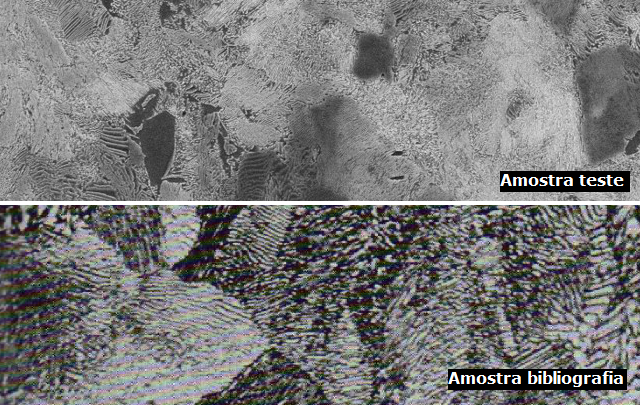
\includegraphics[width=0.7\textwidth]{comparacao_perlita}
\caption{Comparação entre a micrografia obtida e a bibliografia.}
\label{fig:comparacao_perlita}
\end{figure}
\end{frame}

\subsection{Ensaio de Desgaste}

\begin{frame}
	\frametitle{Esquema de teste de cada amostra}
	
	\begin{figure}
		\centering
		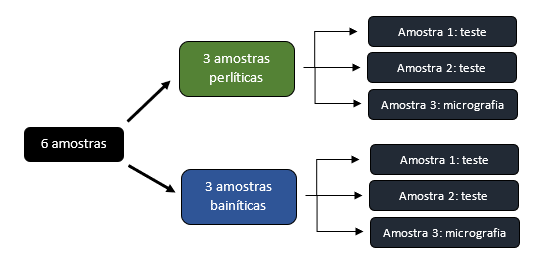
\includegraphics[width=0.8\textwidth]{amostras}
		\caption{Esquema de utilização de cada amostra.}
		\label{fig:amostras}
	\end{figure}
\end{frame}

\begin{frame}
\frametitle{Teste de desgaste}

\begin{columns}[c] % The "c" option specifies centered vertical alignment while the "t" option is used for top vertical alignment
	\column{.4\textwidth} % Left column and width
	


% Table generated by Excel2LaTeX from sheet 'Sheet1'
\begin{table}[H]
	\centering
	\caption{Constantes utilizadas no cálculo da taxa de desgaste.}
	\resizebox{\textwidth}{!}{%
	\begin{tabular}{|cc|}
		\hline
		\multicolumn{2}{|c|}{\textbf{Constantes}} \bigstrut\\
		\hline
		Rotação (n) [rpm] & 433 \bigstrut[t]\\
		Distância do centro (r) [m] & 0,042 \\
		Tempo (t) [h] & 1 \\
		Massa (carga) [kg] & 5 \bigstrut[b]\\
		\hline
	\end{tabular}%
}
	\label{tab:constantes}%
\end{table}%

	
	
	\column{0.6\textwidth} % Right column and width]
	\begin{figure}
		\centering
		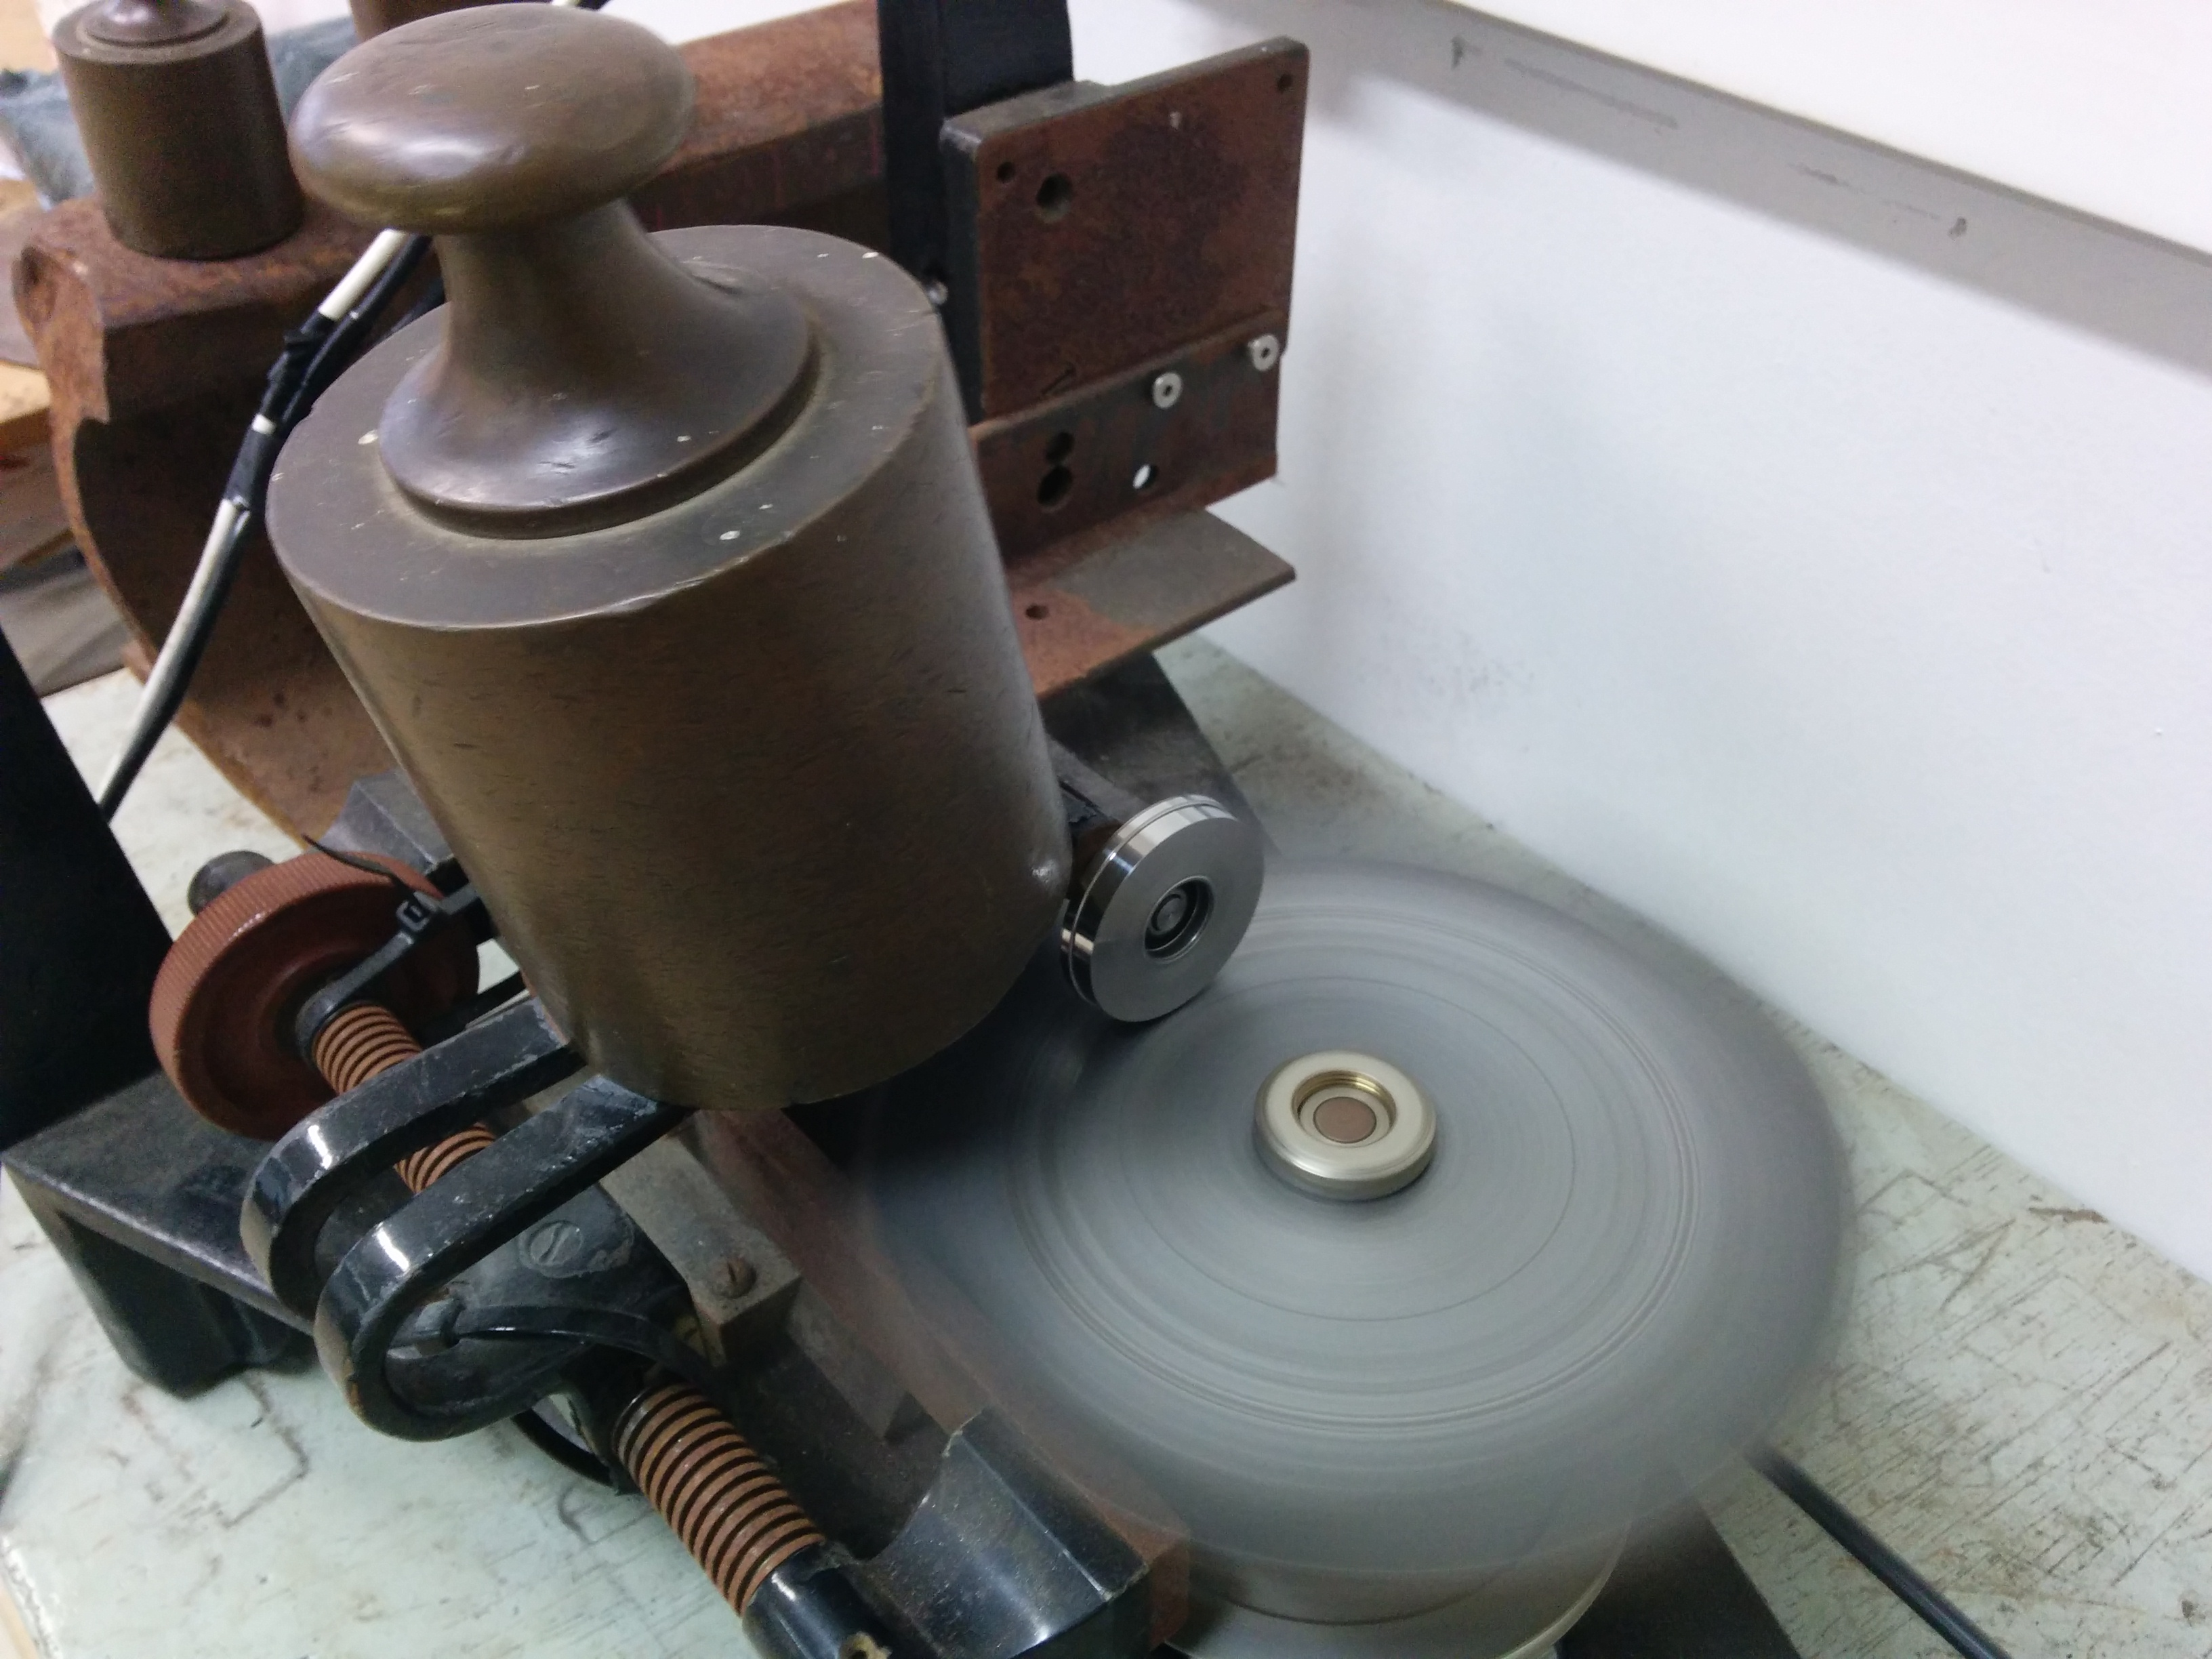
\includegraphics[width=1\textwidth]{tribometro}
		\caption{Amostra em teste no tribômetro.}
		\label{fig:tribometros}
	\end{figure}
	
\end{columns}
\end{frame}



\begin{frame}
\frametitle{Equipamentos para a correta aferição da perda de massa}

\begin{columns}[c] % The "c" option specifies centered vertical alignment while the "t" option is used for top vertical alignment
	\column{.5\textwidth} % Left column and width
	\begin{figure}
		\centering
		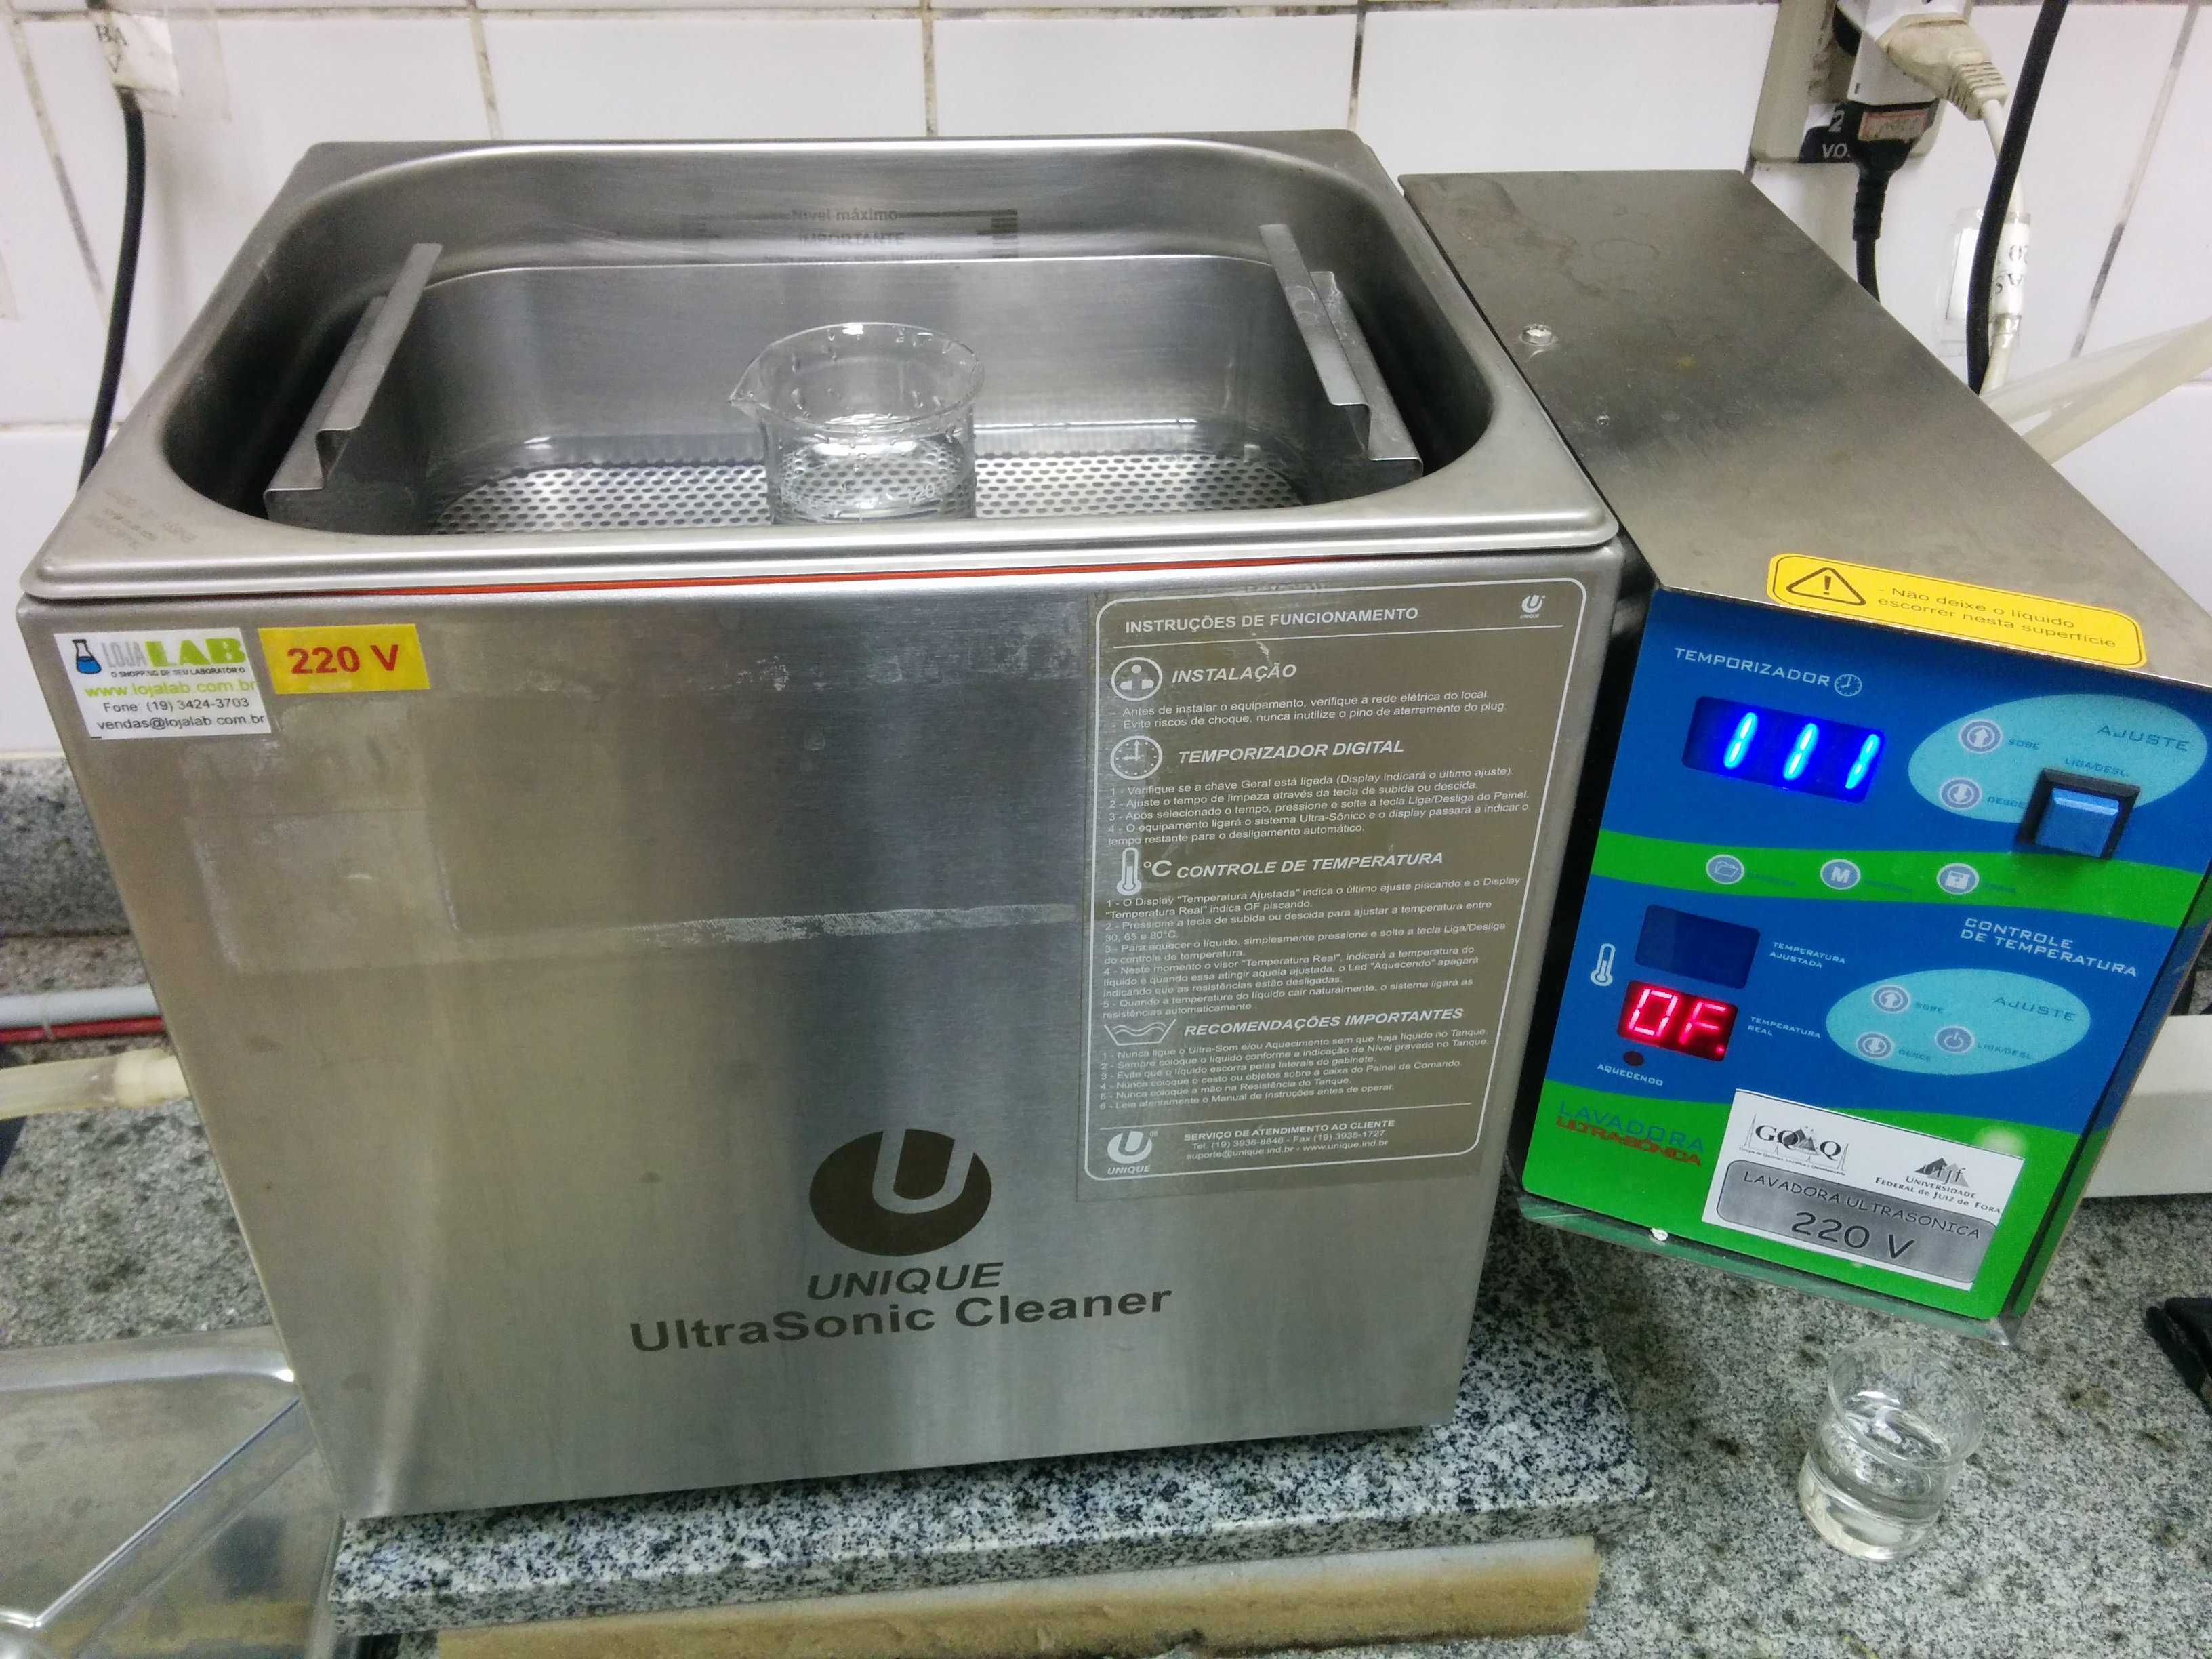
\includegraphics[width=0.9\textwidth]{ultrassom}
		\caption{Ultrassom.}
		\label{fig:ultrassom}
	\end{figure}
	
	
	\column{0.5\textwidth} % Right column and width]
	\begin{figure}
		\centering
		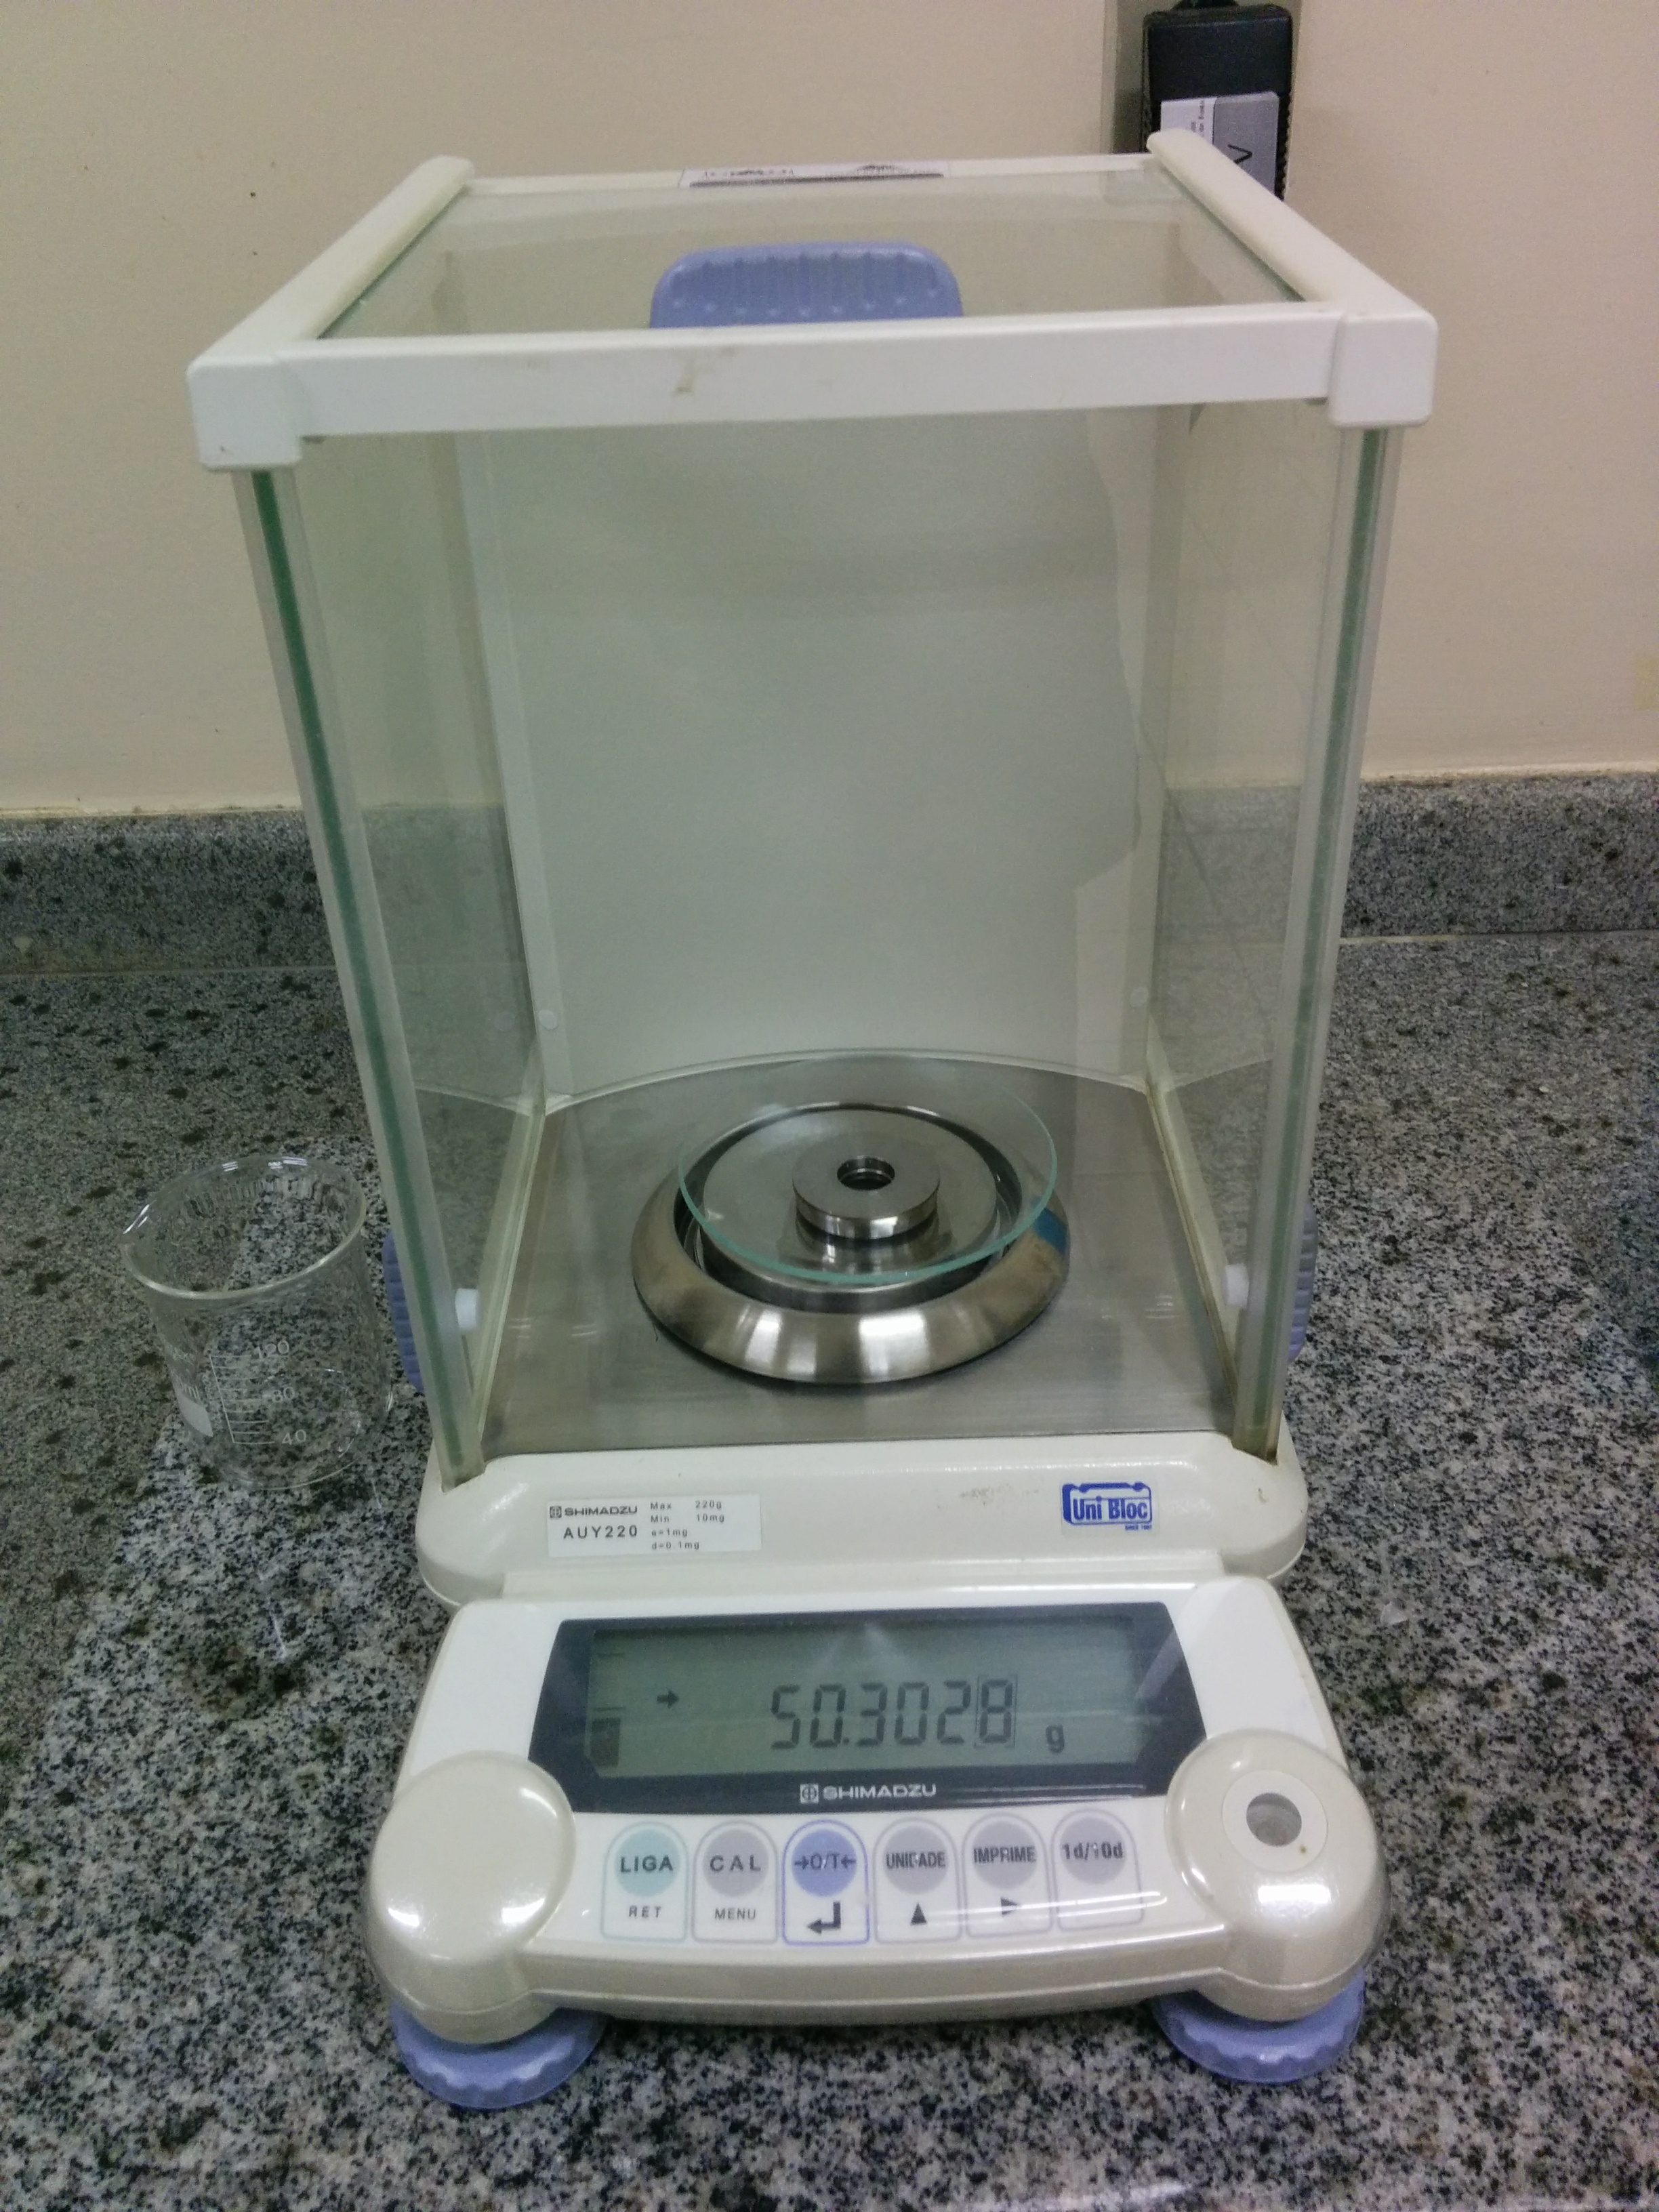
\includegraphics[width=0.6\textwidth]{balanca}
		\caption{Balança analítica.}
		\label{fig:balanca}
	\end{figure}
	
\end{columns}
\end{frame}





%------------------------------------------------

\begin{frame}
\frametitle{Dados obtidos}

\begin{table}[H]
	\centering
	%\caption{Dados de perda de massa e taxa de desgaste obtidos a partir do ensaio de desgaste para a primeira amostra de perlita.}
	\resizebox{0.5\textwidth}{!}{%
		\begin{tabular}{|ccccccc|}
			\hline
			\multicolumn{7}{|c|}{\textbf{Perlita 1}} \bigstrut\\
			\hline
			\multicolumn{1}{|p{3em}}{Carga} & \multicolumn{1}{p{3.5em}}{Leitura} & \multicolumn{1}{p{6.5em}}{Massa da amostra (g)} & \multicolumn{1}{p{6.5em}}{Perda de massa (g)} & \multicolumn{1}{p{7.5em}}{Taxa de desgaste (g.h/m)} & \multicolumn{1}{p{7.5em}}{Taxa de desgaste média (g.h/m)} & \multicolumn{1}{p{7.5em}|}{Desvio padrão (g.h/m)} \bigstrut\\
			\hline
			- & - & 59,7719 & - & - & - & - \bigstrut\\
			\hline
			\multirow{3}[2]{*}{5kg} & 1 & 59,7708 & 0,0011 & 5,78E-04 & \multirow{3}[2]{*}{4,03E-04} & \multirow{3}[2]{*}{2,19E-04} \bigstrut[t]\\
			& 2 & 59,7705 & 0,0003 & 1,58E-04 &   &  \\
			& 3 & 59,7696 & 0,0009 & 4,73E-04 &   &  \bigstrut[b]\\
			\hline
		\end{tabular}%
	}
%	\label{tab:perlita1}%
\end{table}%

% Table generated by Excel2LaTeX from sheet 'Sheet1'
\begin{table}[H]
	\centering
%	\caption{Dados de perda de massa e taxa de desgaste obtidos a partir do ensaio de desgaste para a segunda amostra de perlita.}
	\resizebox{0.5\textwidth}{!}{%
		\begin{tabular}{|ccccccc|}
			\hline
			\multicolumn{7}{|c|}{\textbf{Perlita 2}} \bigstrut\\
			\hline
			\multicolumn{1}{|p{3em}}{Carga} & \multicolumn{1}{p{3.5em}}{Leitura} & \multicolumn{1}{p{6.5em}}{Massa da amostra (g)} & \multicolumn{1}{p{6.5em}}{Perda de massa (g)} & \multicolumn{1}{p{7.5em}}{Taxa de desgaste (g.h/m)} & \multicolumn{1}{p{7.5em}}{Taxa de desgaste média (g.h/m)} & \multicolumn{1}{p{7.5em}|}{Desvio padrão (g.h/m)} \bigstrut\\
			\hline
			- & - & 59,5556 & - & - & - & - \bigstrut\\
			\hline
			\multirow{3}[2]{*}{5kg} & 1 & 59,5538 & 0,0018 & 9,46E-04 & \multirow{3}[2]{*}{5,43E-04} & \multirow{3}[2]{*}{3,58E-04} \bigstrut[t]\\
			& 2 & 59,5533 & 0,0005 & 2,63E-04 &   &  \\
			& 3 & 59,5525 & 0,0008 & 4,20E-04 &   &  \bigstrut[b]\\
			\hline
		\end{tabular}%
	}
%	\label{tab:perlita2}%
\end{table}%







% Table generated by Excel2LaTeX from sheet 'Sheet1'
\begin{table}[H]
	\centering
	%\caption{Dados de perda de massa e taxa de desgaste obtidos a partir do ensaio de desgaste para a primeira amostra de bainita.}
	\resizebox{0.5\textwidth}{!}{%
		\begin{tabular}{|ccccccc|}
			\hline
			\multicolumn{7}{|c|}{\textbf{Bainita 1}} \bigstrut\\
			\hline
			\multicolumn{1}{|p{3em}}{Carga} & \multicolumn{1}{p{3.5em}}{Leitura} & \multicolumn{1}{p{6.5em}}{Massa da amostra (g)} & \multicolumn{1}{p{6.5em}}{Perda de massa (g)} & \multicolumn{1}{p{7.5em}}{Taxa de desgaste (g.h/m)} & \multicolumn{1}{p{7.5em}}{Taxa de desgaste média (g.h/m)} & \multicolumn{1}{p{7.5em}|}{Desvio padrão (g.h/m)} \bigstrut\\
			\hline
			- & - & 53,4592 & - & - & - & - \bigstrut\\
			\hline
			\multirow{3}[2]{*}{5kg} & 1 & 53,4581 & 0,0011 & 5,78E-04 & \multirow{3}[2]{*}{8,76E-04} & \multirow{3}[2]{*}{2,70E-04} \bigstrut[t]\\
			& 2 & 53,456 & 0,0021 & 1,10E-03 &   &  \\
			& 3 & 53,4542 & 0,0018 & 9,46E-04 &   &  \bigstrut[b]\\
			\hline
		\end{tabular}%
	}
%	\label{tab:bainita1}%
\end{table}%

% Table generated by Excel2LaTeX from sheet 'Sheet1'
\begin{table}[H]
	\centering
%	\caption{Dados de perda de massa e taxa de desgaste obtidos a partir do ensaio de desgaste para a segunda amostra de bainita.}
	\resizebox{0.5\textwidth}{!}{%
		\begin{tabular}{|ccccccc|}
			\hline
			\multicolumn{7}{|c|}{\textbf{Bainita 2}} \bigstrut\\
			\hline
			\multicolumn{1}{|p{3em}}{Carga} & \multicolumn{1}{p{3.5em}}{Leitura} & \multicolumn{1}{p{6.5em}}{Massa da amostra (g)} & \multicolumn{1}{p{6.5em}}{Perda de massa (g)} & \multicolumn{1}{p{7.5em}}{Taxa de desgaste (g.h/m)} & \multicolumn{1}{p{7.5em}}{Taxa de desgaste média (g.h/m)} & \multicolumn{1}{p{7.5em}|}{Desvio padrão (g.h/m)} \bigstrut\\
			\hline
			- & - & 50,3032 & - & - & - & - \bigstrut\\
			\hline
			\multirow{3}[2]{*}{5kg} & 1 & 50,3028 & 0,0004 & 2,10E-04 & \multirow{3}[2]{*}{2,63E-04} & \multirow{3}[2]{*}{5,25E-05} \bigstrut[t]\\
			& 2 & 50,3023 & 0,0005 & 2,63E-04 &   &  \\
			& 3 & 50,3017 & 0,0006 & 3,15E-04 &   &  \bigstrut[b]\\
			\hline
		\end{tabular}%
	}
	%\label{tab:bainita2}%
\end{table}%

\end{frame}

%------------------------------------------------





%----------------------------------------------------------------------------------------
\section{Resultados e Análises}

\begin{frame}
\frametitle{Gráfico dos dados de desgaste}
\begin{figure}
	\centering
	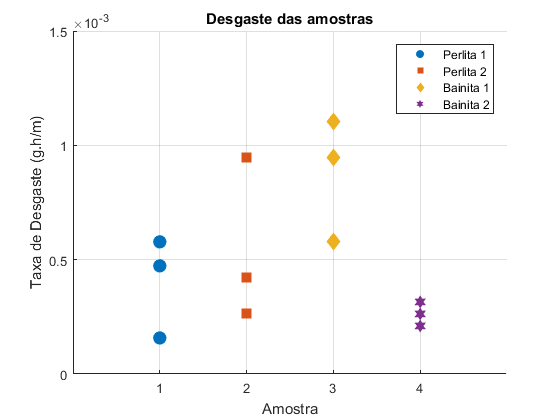
\includegraphics[width=0.8\textwidth]{graf1}
	\caption{Reprodução dos dados de desgaste obtidos a partir do ensaio de desgaste em forma de gráfico.}
	\label{fig:graf1}
\end{figure}
\end{frame}

\begin{frame}
\frametitle{Análise}
\begin{itemize}
	\item As taxas de desgaste apresentaram valores bastante variáveis, mesmo quando analisando cada amostra individualmente.
	\item Não há constância de valores, com exceção da amostra Bainita 2. 
	\item Mesmo dentro da mesma categoria de microestrutura os resultados são divergentes.
\end{itemize}

\end{frame}

\begin{frame}
\frametitle{Média dos testes e desvio padrão}
\begin{figure}
	\centering
	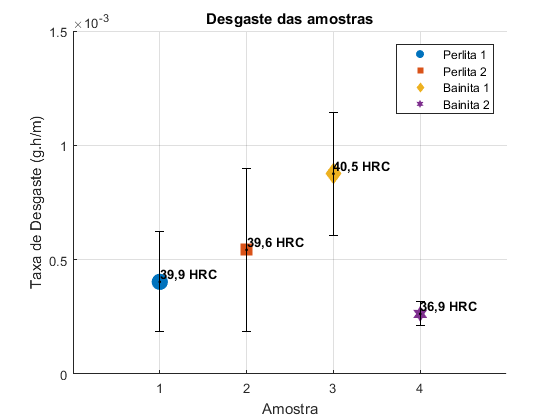
\includegraphics[width=0.8\textwidth]{graf2}
	\caption{Gráfico da média dos testes de cada amostra com barras representando o desvio padrão das taxas de desgastes individuais. Os números próximos aos símbolos representam a dureza de cada amostra.}
	\label{fig:graf2}
\end{figure}
\end{frame}

\begin{frame}
\frametitle{Análise}
\begin{itemize}
	\item Alto desvio padrão para todas as amostras, exceto para a amostra Bainita 2
	\item Resultados não satisfatórios a fim de comparação das duas microestruturas.
\end{itemize}

\end{frame}

%------------------------------------------------
\section{Conclusões}


\begin{frame}
	A partir das análises dos resultados dos gráficos é possível deduzir que o método de avaliação de desgaste adotado neste trabalho de pesquisa não é adequado. 
\begin{itemize}
	\item Tal inconformidade de resultados pode ter ocorrido pelos seguintes motivos:
\end{itemize}

\end{frame}

\begin{frame}
\begin{block}{A carga aplicada entre o contato roda-trilho é muito baixa}
	A espessura da área de rolamento foi reduzida a 2 mm através usinagem de chanfros na pista de rolamento e a carga utilizada foi a do peso de 5 kg, maior peso disponível no laboratório para o tribômetro. Apesar disso, as tensões impostas nos corpos de provas, mesmo em miniaturas, são muito inferiores a tais percebidas em aplicações reais no transporte de minério de ferro. Com tensões próximas às tensões reais, as perdas de massa seriam bem mais significativas.
\end{block}

\end{frame}

\begin{frame}
\begin{block}{A balança não pode captar somente a perda de massa devido ao desgaste}
	As aferições de massa foram realizadas em balanças analíticas, com precisão de 0,0001 g. Todavia, é possível que as perdas de massa por desgaste para a carga aplicada sejam tão ínfimas que não possam ser perfeitamente captadas pela balança.
\end{block}

\end{frame}

\begin{frame}
\begin{block}{O ambiente externo interfere na massa da amostra}
	Como as perdas de massa são muito pequenas, a própria interação do ambiente com o corpo de prova pode alterar sua massa. Tal interação prejudica a observação da perda de massa por desgaste. Apesar de ser sido realizada a lavagem ultrassônica em todos os corpos de prova antes da aferição de massa, a amostra pode, com mais ou menos intensidade, ter adquirido partículas do ar ou dos dedos do manuseador no deslocamento da lavadora até a balança. Além disso, outro fenômeno de interação com o ambiente que ocorre e pode resultar em alterações de massa é a oxidação gradual do metal com o ar atmosférico.
\end{block}

\end{frame}

\begin{frame}
\begin{block}{O tempo de rolamento não é suficiente}
	O intervalo de teste adotado no tribômetro foi de 1 hora. Esse intervalo de tempo pode não ser suficiente para uma perda de massa por desgaste significativa. Uma maior perda de massa por desgaste através do aumento do tempo de teste reduziria a influência de outras variáveis na variação da massa.
\end{block}

\end{frame}

\begin{frame}
\begin{block}{Desgaste de forma aleatória}
	O fenômeno de desgaste ocorreu de forma não linear. As massas perdidas através das tensões do contato roda-trilho não são constantes. Detritos maiores podem se quebrar da amostra de forma repentina, assim como durante um longo intervalo pode nenhuma partícula se soltar. Para reduzir esses efeitos na avaliação do real desgaste, longos intervalos de tempo de testes seriam necessários.
\end{block}

\end{frame}



\begin{frame}
\Huge{\centerline{Obrigado}}
\end{frame}

\end{document} 